% NetDream: NeurIPS 2026 Submission
% Contribution type: Use-Inspired
% Subject area: SysML Infrastructure
%

\documentclass{article}
\usepackage{neurips_2025}  % Will update to neurips_2026 when available

\usepackage[utf8]{inputenc}
\usepackage[T1]{fontenc}
\usepackage{hyperref}
\usepackage{url}
\usepackage{booktabs}
\usepackage{amsfonts}
\usepackage{amsmath}
\usepackage{nicefrac}
\usepackage{microtype}
\usepackage{graphicx}
\usepackage{xcolor}
\usepackage{enumitem}
\usepackage{algorithm}
\usepackage{algorithmic}
\usepackage{subcaption}
\usepackage{multirow}
\usepackage{float}
\usepackage{amsthm}
\usepackage{dsfont}
\usepackage{pifont}
\newtheorem{proposition}{Proposition}
\newcommand{\cmark}{\ding{51}}
\newcommand{\xmark}{\ding{55}}

% NeurIPS checklist answer commands
\newcommand{\answerYes}[1]{\textbf{Yes.} #1}
\newcommand{\answerNo}[1]{\textbf{No.} #1}
\newcommand{\answerNA}[1]{\textbf{N/A.} #1}

\title{Autoscaling by Imagination: Graph World Models for Safe Distributed Machine Learning Services}

\author{
  Anonymous Author(s)
}

\begin{document}
\maketitle

\begin{abstract}
Modern machine learning services are increasingly deployed as distributed microservice systems, where resource allocation decisions must balance latency, reliability, and cost. In practice, however, autoscaling remains largely reactive: controllers add replicas only after the system is already under pressure, while safer deployments often rely on static over-allocation. Existing autoscalers do not learn a model of how scaling actions propagate through the service graph, and therefore cannot anticipate how a decision will affect future load, latency, cost, and service-level violations before it is executed. To fill this research gap, we present \emph{NetDream}, a graph world model for safe autoscaling of distributed machine learning services. NetDream learns action-conditioned dynamics over a microservice graph, predicting how load, latency, replicas, and violation risk evolve under candidate scaling actions. At runtime, NetDream uses this learned model for imagination-based planning: it rolls out multiple future scaling trajectories, filters out plans predicted to violate service-level constraints, and executes the first action of the best safe plan. This turns autoscaling from threshold-based reaction into topology-aware planning over a learned model of the system. We evaluate NetDream on a production-grade AWS Kubernetes deployment of Online Boutique, an 11-service, 14-edge microservice graph with a 66-dimensional system state and 48,000 collected transitions, under steady, variable, bursty, and flash-crowd traffic. NetDream-Safe is the most cost-efficient safe autoscaler among all evaluated methods. Each marginal replica-step it spends buys safety $2.7\times$ more cost-efficiently than the best static over-provisioning strategy. On variable-traffic workloads specifically, it achieves about $5\times$ fewer violations than standard reactive autoscaling while using only about half the cost of the strongest static over-provisioning baseline; on flash-crowd traffic the gain narrows because pod-startup delay bottlenecks all autoscalers. Finally, removing graph structure makes one-step prediction $11\times$ worse, showing that graph structure is required for reliable multi-step prediction. Code, trained models, infrastructure manifests, and a 30-second explainer video are released anonymously at \url{https://anonymous.4open.science/r/netdream-FCF9}.

\end{abstract}

\section{Introduction}
\label{sec:intro}

Modern machine learning services are increasingly deployed as distributed
microservice systems~\citep{qiu2020firm,alibabatrace2022}. A single user
request may pass through many interacting components: frontend services,
retrieval services, ranking services, payment or logging services,
caches, databases, and model serving endpoints. Keeping such systems
reliable requires continuous resource allocation. Too few replicas lead
to latency spikes and service-level violations; too many replicas waste
compute. Autoscaling is therefore a core control problem for distributed
machine learning services: decide where to add or remove capacity, under
changing demand, while balancing latency, reliability, and cost.

Production autoscaling, however, remains largely reactive. Standard
controllers such as the Kubernetes Horizontal Pod Autoscaler
\citep{rzadca2020autopilot,googlecloud2025hpa,aws2025hpa} scale only
after utilization or latency signals indicate that the system is already
under pressure. Recent extensions augment HPA with short-horizon
forecasting or adaptive thresholds
\citep{pozdniakova2024sla,mondal2023predictive,ahmad2024smarthpa,santos2024gwydion},
yet still trigger scaling rules from a forecast metric rather than from
a simulated future trajectory. Safer deployments often compensate by
keeping extra replicas alive at all times. This creates a familiar but unsatisfactory trade-off: reactive
scaling is cheap but late, while static over-allocation is safer but
expensive. The problem is not only that existing controllers use simple
thresholds. More fundamentally, they act without a learned model of
the system: they do not know how a scaling action will propagate
through the service graph, how it will change downstream load and
latency, or whether it will create a future service-level violation.

We will refer to this missing capability as \emph{imagination}: the
ability of an autoscaler to ask counterfactual questions before acting,
in the spirit of learned world models that have proven effective for
planning in other domains~\citep{ha2018worldmodels,hafner2025dreamerv3}.
If we add replicas to the frontend, will the bottleneck move to checkout? If we scale the
recommendation service, will latency improve or will traffic shift to
the product catalog service? If we reduce capacity now, will the system
remain safe over the next few control steps? Current autoscalers mostly
act, observe, and correct. They do not simulate the consequences of their
actions before those actions reach the real cluster.

\begin{figure*}[t]
\centering
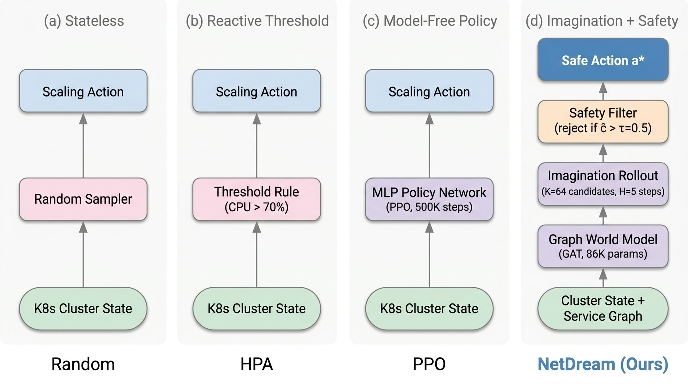
\includegraphics[width=\textwidth]{figures/fig_motivation.pdf}
\caption{\textbf{Why NetDream.}
Existing Kubernetes autoscalers map the current cluster state directly
to a scaling action: \textbf{(a)}~Random samples uniformly,
\textbf{(b)}~HPA reacts when CPU crosses a threshold, and
\textbf{(c)}~PPO learns a model-free policy. None of them imagine
future states before acting. \textbf{(d)}~NetDream inserts a graph
world model and a safety filter into this loop, so that candidate
scaling actions are first rolled out in imagination, scored, and
rejected if they are predicted to violate service-level constraints.}
\label{fig:motivation}
\end{figure*}

To answer the above questions and fill the research gap, we present
NetDream, a graph world model for safe autoscaling of distributed
machine learning services. NetDream represents a microservice
application as a graph, where nodes are services and edges are
service-call dependencies. While prior work has applied graph neural
networks to predict tail latency~\citep{park2021graf} or to learn
model-free actor--critic policies for autoscaling~\citep{chen2025graphpilot},
and digital-twin approaches~\citep{karma2025} have built unstructured
neural transition models of clusters, NetDream is, to our knowledge, the
first to combine a graph-structured dynamics model with imagination-based
planning and an explicit safety filter. It learns action-conditioned dynamics over
this graph: given the current service states and a candidate scaling
action, the model predicts how load, latency, replicas, reward, and
violation risk will evolve. At runtime, NetDream uses this learned model
inside an imagination-based planner. The planner rolls out multiple
future scaling trajectories, rejects those predicted to violate
service-level constraints, and executes only the first action of the best
safe plan. In this way, NetDream turns autoscaling from threshold-based
reaction into topology-aware planning over a learned model of the
system.

This formulation is operationally practical.
NetDream does not require an online reinforcement-learning agent to
explore risky actions in the real cluster~\citep{qiu2023aware,zhang2025kiss}.
Instead, it learns from logged transitions and uses the learned world
model as a simulator for planning.
The safety mechanism is also explicit: candidate futures whose predicted
violation risk exceeds a threshold are filtered out before execution.
This makes the controller closer to how human operators reason about
infrastructure: compare possible actions, reject unsafe ones, and choose
the lowest-cost safe plan.

\begin{figure*}[t]
\centering
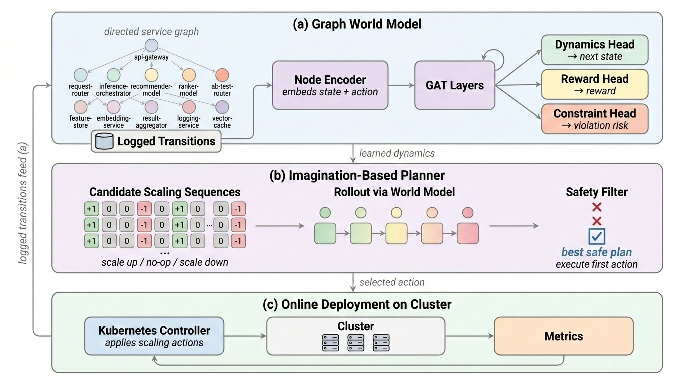
\includegraphics[width=\textwidth]{figures/fig_overview.pdf}
\caption{\textbf{NetDream for safe autoscaling of distributed machine
learning services.}
NetDream learns a graph world model of a microservice application
(illustrated here on a representative ML serving graph: api-gateway,
inference-orchestrator, recommender / ranker / embedding services,
feature store, etc.). Given the current service states and candidate
scaling actions, the model predicts future state changes, reward, and
service-level violation risk. A planning module rolls out multiple
candidate action sequences in imagination, rejects unsafe futures
through a learned safety filter, and executes the first action of the
best safe plan. Our empirical evaluation (Section~\ref{sec:experiments})
follows the standard Kubernetes autoscaling benchmarking practice and
uses Google's Online Boutique~\citep{googlecloud2023onlineboutique} —
the 11-service / 14-edge testbed adopted by recent GNN-based autoscaling
work~\citep{park2021graf,meng2023deepscaler,chen2025graphpilot} —
as a topologically equivalent representative of this microservice
class.}
\label{fig:overview}
\end{figure*}

We evaluate NetDream on a production-grade AWS Kubernetes deployment of
Online Boutique~\citep{googlecloud2023onlineboutique}, an 11-service,
14-edge microservice graph with a 66-dimensional system state and
48,000 collected transitions. The autoscaler is stress-tested under
four workload regimes (steady traffic, variable demand, bursty spikes,
and flash crowds) generated with Locust~\citep{locust} and replayed
from production microservice traces~\citep{alibabatrace2022}. We compare against
standard reactive autoscaling, static over-provisioning strategies,
random scaling, model-free reinforcement learning, and an ablation of
NetDream without the safety filter.

Our results show that graph-world-model planning is a more cost-efficient
path to safe autoscaling than reactive control or static
over-provisioning. NetDream-Safe sits on the cost--safety Pareto frontier
on a real AWS EKS deployment, and removing graph structure degrades
one-step prediction by $11\times$. We defer the per-workload numbers
and ablations to Section~\ref{sec:experiments}, and provide cross-domain
validation (power grid, water network, epidemic mobility graph) as
supplementary evidence that the architecture is not Kubernetes-specific
in Appendix~\ref{app:generalizability}.

Overall, this paper makes three contributions:

\begin{itemize}
\item We formulate autoscaling for distributed machine learning services
as planning with a learned graph world model. Instead of reacting to
threshold crossings, NetDream predicts the multi-step consequences of
scaling actions across the service graph before execution.

\item We introduce an imagination-based safety filter for autoscaling.
The planner rolls out candidate scaling sequences inside the learned
world model and rejects plans predicted to cause future service-level
violations.

\item We demonstrate cost-efficient safe autoscaling on a real AWS
Kubernetes deployment. On the Online Boutique benchmark, NetDream
achieves substantially better cost--safety trade-offs than reactive
autoscaling, static over-provisioning, model-free reinforcement learning,
and unsafe planning ablations.
\end{itemize}
\section{Related Works}
\label{sec:related}
\if0
NetDream sits at the intersection of Kubernetes autoscaling and learned
control.  The closest prior systems recognize either that autoscaling
should be predictive, or that microservice systems should be modeled as
graphs.  Our distinction is that NetDream uses a graph-structured world
model not only to predict a future metric, but to plan over imagined
future system trajectories and reject unsafe actions before execution.

\subsection{From Reactive Autoscaling to Predictive Kubernetes Control}
\label{sec:related-reactive-predictive}

Production Kubernetes autoscaling is still dominated by reactive control.
The Horizontal Pod Autoscaler (HPA) scales replica counts when CPU
utilization or custom metrics cross a configured threshold
\citep{rzadca2020autopilot,googlecloud2025hpa,aws2025hpa}.  This design
is simple, robust, and easy to operate, which explains its broad
adoption.  Its limitation is also fundamental: HPA observes pressure only
after it appears.  It cannot predict whether scaling one service will
shift load to another service, reduce downstream latency, or create a
future service-level violation.

A line of work augments HPA with forecasting or adaptive rules.
SLA-adaptive HPA dynamically adjusts thresholds
\citep{pozdniakova2024sla}; Predictive HPA forecasts demand several
minutes ahead \citep{mondal2023predictive}; Smart HPA uses recurrent
time-series models \citep{ahmad2024smarthpa}; TAHPA exploits diurnal
patterns \citep{phuc2022tahpa}; and Gwydion switches between reactive
and predictive modes \citep{santos2024gwydion}.  These methods improve
when the workload has predictable temporal structure, but they remain
limited by the same control interface: forecast a metric, then trigger a
rule.  They do not learn a transition model of the microservice graph,
nor do they simulate the multi-step consequences of candidate scaling
actions before acting.

NetDream takes a different view.  Autoscaling is not merely forecasting
future load; it is choosing among counterfactual futures.  The controller
must ask what will happen if it scales the frontend, the checkout
service, or the recommendation service, and how each action will affect
latency, cost, and violations over the next several control steps.
NetDream addresses this by learning an action-conditioned graph world
model and using it inside a planner.  This turns predictive autoscaling
from metric forecasting into model-based decision making.

\subsection{Learning-Based Autoscaling: From Metric Prediction to World Models}
\label{sec:related-learning-autoscaling}

\paragraph{Reactive Kubernetes autoscaling.}
Production autoscaling is still dominated by Kubernetes' Horizontal Pod
Autoscaler (HPA), which scales replicas once CPU or custom-metric
utilization crosses a configured threshold
\citep{rzadca2020autopilot,googlecloud2025hpa,aws2025hpa}.
HPA is simple and operationally proven but cannot anticipate downstream
load, predict latency cascades, or simulate the multi-step consequences
of a scaling decision.
Variants that augment HPA with short-horizon demand forecasting
\citep{mondal2023predictive,ahmad2024smarthpa,santos2024gwydion} or
adaptive thresholds
\citep{pozdniakova2024sla,phuc2022tahpa}
improve responsiveness when traffic has predictable temporal structure,
but they still trigger scaling rules from a forecast metric rather than
from a simulated future trajectory.

\paragraph{Topology-aware prediction and model-free control.}
\fi

Learning-based autoscaling has moved beyond hand-designed rules, but
most methods still fall into two categories: predict a metric and react,
or learn a policy directly.  GNN-based autoscalers exploit the fact that
microservice systems are graphs.  GRAF predicts tail latency with a GNN
and uses the prediction for proactive SLO-aware allocation
\citep{park2021graf}.  pHPA continuously trains a GNN to infer tail
latency along microservice chains \citep{choi2021phpa}.  DeepScaler
combines spatio-temporal GNNs with adaptive graph learning for holistic
autoscaling \citep{meng2023deepscaler}; Graph-PHPA combines LSTM and GNN
modules for proactive horizontal scaling \citep{dang2022graphphpa}; AGQ
uses dense spatio-temporal GNNs to capture indirect dependencies
\citep{liang2025agq}; and USRFNet learns unified system representations
for microservice tail-latency prediction \citep{zhang2025usrfnet}.  These
systems show that topology-aware representations matter, but their
control logic remains prediction-driven rather than imagination-driven:
the GNN predicts a future metric, and a separate heuristic or policy
decides how to scale. Reinforcement-learning autoscalers instead learn control policies
directly.  Prior work has explored DQN, PPO, TD3, and recurrent
reinforcement learning for microservice and serverless autoscaling
\citep{abdelkhaleq2023dqn,qiu2023aware,zhang2025kiss,drpc2024,
agarwal2024deep}.  Multi-objective variants optimize SLO and cost
trade-offs through bi-level control, Lagrangian relaxation, or Pareto
optimization \citep{wang2024autothrottle,wang2024deepscaling,
marchese2025slocost}.  GraphPilot is closest in spirit among GNN-based
controllers: it combines a Temporal Graph Network encoder with an
actor--critic policy for Kubernetes autoscaling
\citep{chen2025graphpilot}.  However, these approaches learn a policy,
not a graph world model used for explicit planning.  They do not roll out
candidate action sequences in a learned dynamics model and reject unsafe
futures before execution. Digital-twin approaches move closer to model-based control. KARMA builds
a neural transition model of the cluster and trains multi-agent policies
in simulation for resilience against failures such as DDoS attacks and
pod crashes \citep{karma2025}.  However, its transition model is not
graph-structured, and its objective is adversarial resilience rather than
cost--SLO autoscaling on standard microservice workloads. 
NetDream differs in three ways: it learns topology-aware graph dynamics, uses the learned model online for model-predictive planning, and applies an
explicit safety filter that rejects candidate action sequences predicted
to violate service-level constraints. 
In summary, prior Kubernetes autoscalers either react to observed
pressure, forecast a metric and apply a rule, or learn a model-free
policy. NetDream instead treats autoscaling as planning with a learned
graph world model.  This distinction is the source of its empirical
advantage: the controller can compare multiple possible futures, reason
over service dependencies, and avoid unsafe plans before they are applied
to the real cluster.
\section{Method}
\label{sec:method}

NetDream is built on one idea: safe autoscaling requires a model of the
future. Instead of reacting to threshold crossings, NetDream learns a
graph world model of a Kubernetes microservice application, uses it to
imagine the consequences of candidate scaling actions, rejects unsafe
futures, and executes the first action of the best safe plan. This
section formalises the control problem
(Section~\ref{sec:formulation}), specifies the graph world model
(Section~\ref{sec:world-model}), describes imagination-based planning
with the safety filter (Section~\ref{sec:planning}), and summarises how
the trained model is deployed on a real Kubernetes cluster
(Section~\ref{sec:deployment}).

\subsection{Problem Formulation}
\label{sec:formulation}

We represent a Kubernetes application as a directed service graph
$\mathcal{G}=(V,E)$, where each node $i\in V$ is a microservice and each
edge $(i,j)\in E$ is a service-call dependency. At control step $t$,
service $i$ has state
\[
x_{t,i} =
[\mathrm{CPU}_{t,i}, \mathrm{memory}_{t,i}, \mathrm{QPS}_{t,i},
\mathrm{latency}_{t,i}, \mathrm{error}_{t,i}, \mathrm{replicas}_{t,i}]
\in \mathbb{R}^{d}.
\]
The full cluster state is
\[
X_t = [x_{t,1},\ldots,x_{t,N}] \in \mathbb{R}^{N\times d}.
\]

The autoscaler chooses a per-service scaling action
\[
A_t=[a_{t,1},\ldots,a_{t,N}], \qquad a_{t,i}\in\{-1,0,+1\},
\]
corresponding to scaling service $i$ down, holding it fixed, or scaling
it up by one replica. After the action is applied, the cluster evolves
to $X_{t+1}$, receives reward $r_t$, and may incur a service-level
violation $c_t\in\{0,1\}$. The true transition process
\[
X_{t+1}\sim T(X_t,A_t;\mathcal{G})
\]
is unknown and difficult to model analytically because it depends on
request routing, queueing, pod startup delays, workload shifts, and
cross-service dependencies.

The objective is to reduce service-level violations while avoiding
unnecessary replica cost. We use a reward that penalizes both resource
usage and violations:
\[
r_t =
-\lambda_{\mathrm{cost}}\mathrm{Cost}(X_t)
-\lambda_{\mathrm{slo}}c_t,
\qquad
\mathrm{Cost}(X_t)
=
\sum_{i=1}^{N}\mathrm{replicas}_{t,i},
\]
where the violation indicator $c_t = \mathds{1}[\,\exists\,i\in V :
\mathrm{latency}_{t+1,i}>\mathrm{SLO}\,]$ flags whether the transition
into $X_{t+1}$ produced an SLO breach at any service.
However, NetDream does not rely on reward optimization alone. It also
learns an explicit constraint predictor and uses it during planning to
discard unsafe futures before they are executed.

\subsection{Graph World Model}
\label{sec:world-model}

NetDream learns an action-conditioned graph world model
\[
f_\theta(\mathcal{G},X_t,A_t)
\rightarrow
(\Delta\hat{X}_t,\hat{r}_t,\hat{c}_t),
\]
where $\Delta\hat{X}_t$ is the predicted state residual, $\hat{r}_t$ is
the predicted reward, and $\hat{c}_t$ is the predicted probability of a
service-level violation. The next state is predicted as
\[
\hat{X}_{t+1}=X_t+\Delta\hat{X}_t .
\]
Residual prediction makes the model focus on short-term changes rather
than reconstructing absolute state, which is important for stable
multi-step rollouts.

For each service, NetDream first encodes the current state and candidate
scaling action. Because $a_{t,i}\in\{-1,0,+1\}$ is categorical, we
one-hot encode it before concatenation:
\[
h^{(0)}_{t,i}
=
\phi_{\mathrm{enc}}\left(\bigl[x_{t,i}\,\bigl\|\,
\mathrm{onehot}(a_{t,i})\bigr]\right),
\qquad
\mathrm{onehot}(a_{t,i})\in\{0,1\}^{3}.
\]
This makes the model counterfactual: it can predict what would happen
under different possible scaling actions, not merely forecast the next
state under the current policy.

NetDream then applies $L$ layers of graph attention over the service-call
topology. The directed call graph $\mathcal{G}$ is symmetrized for
message passing so that downstream load and upstream backpressure can
both flow along an edge; we write $\mathcal{N}(i)$ for the resulting
undirected neighbourhood of service $i$.
\[
\tilde{h}^{(\ell+1)}_{t,i}
=
\mathrm{GAT}^{(\ell)}
\left(
h^{(\ell)}_{t,i},
\{h^{(\ell)}_{t,j}:j\in\mathcal{N}(i)\}
\right),
\qquad
h^{(\ell+1)}_{t,i}
=
h^{(\ell)}_{t,i}+\tilde{h}^{(\ell+1)}_{t,i}.
\]
Message passing lets the model capture how load, latency, and failures
propagate across connected services. Attention is useful because service
dependencies are heterogeneous: scaling one service may strongly affect
some downstream services while barely affecting others.

The final node embeddings are decoded by three heads. The dynamics head
predicts per-service residual state change:
\[
\Delta\hat{x}_{t,i}=\phi_{\mathrm{dyn}}(h^{(L)}_{t,i}).
\]
The reward and constraint heads operate on a graph-level representation
\[
g_t=\mathrm{READOUT}\left(\{h^{(L)}_{t,i}\}_{i=1}^{N}\right),
\]
where $\mathrm{READOUT}$ is mean pooling, yielding
\[
\hat{r}_t=\phi_{\mathrm{rew}}(g_t),
\qquad
\hat{c}_t=\sigma(\phi_{\mathrm{con}}(g_t)).
\]
Thus, the same world model predicts how the system evolves, how costly
the transition is, and whether the future is unsafe.

\paragraph{Training the world model.}
The world model is trained offline from logged Kubernetes transitions
$(\mathcal{G},X_t,A_t,X_{t+1},r_t,c_t)$ by minimising a multi-task
objective:
\[
\mathcal{L}(\theta)
=
\underbrace{
\left\|
f_{\theta}^{\mathrm{dyn}}(\mathcal{G},X_t,A_t)
-
(X_{t+1}-X_t)
\right\|_2^2
}_{\text{state dynamics}}
+
\alpha
\underbrace{
(\hat{r}_t-r_t)^2
}_{\text{reward}}
+
\beta
\underbrace{
\mathrm{BCE}(\hat{c}_t,c_t)
}_{\text{constraint}} .
\]
We use $\alpha=\beta=0.1$, keeping dynamics prediction as the dominant
learning signal while still learning reward and safety estimates for
planning. Instead of learning a policy directly through trial and error,
NetDream first learns how the cluster responds to actions; the learned
model then becomes a simulator for planning. This avoids unsafe online
exploration in the real cluster and makes the controller inspectable:
predictions, rewards, and violation risks are explicit quantities that
can be evaluated before action execution.

\subsection{Imagination-Based Planning}
\label{sec:planning}

At deployment time, NetDream uses the learned world model for
model-predictive control. Given the current state $X_t$, the planner
samples $K$ candidate action sequences of horizon $H$:
\[
\mathbf{A}^{(k)}_{t:t+H-1}
=
(A^{(k)}_t,\ldots,A^{(k)}_{t+H-1}),
\qquad k=1,\ldots,K .
\]
Each sequence is rolled out inside the world model:
\[
\hat{X}^{(k)}_{t+h+1}
=
\hat{X}^{(k)}_{t+h}
+
f_{\theta}^{\mathrm{dyn}}
(\mathcal{G},\hat{X}^{(k)}_{t+h},A^{(k)}_{t+h}),
\]
while also predicting rewards and violation probabilities
$\hat{r}^{(k)}_{t+h}$ and $\hat{c}^{(k)}_{t+h}$. The predicted return of
a candidate plan is
\[
J^{(k)}
=
\sum_{h=0}^{H-1}
\gamma^h \hat{r}^{(k)}_{t+h}.
\]

Before selecting the best plan, NetDream applies an imagination-based
safety filter. A candidate sequence is accepted only if its predicted
violation probability remains below threshold $\tau$ at every imagined
step:
\[
\max_{0\le h < H}\hat{c}^{(k)}_{t+h}\le \tau .
\]
Let $\mathcal{K}_{\mathrm{safe}}$ denote the set of candidates that pass
this filter. NetDream selects
\[
k^*=\arg\max_{k\in\mathcal{K}_{\mathrm{safe}}} J^{(k)}
\]
and executes only the first action $A^{(k^*)}_t$ in the real cluster. If
no candidate is predicted safe, the controller falls back to a
conservative no-op action. After observing the next real cluster state,
NetDream replans. Algorithm~\ref{alg:netdream} summarises the loop.

\begin{algorithm}[t]
\caption{NetDream: Imagination-Based Safe Autoscaling}
\label{alg:netdream}
\begin{algorithmic}[1]
\STATE \textbf{Input:} graph $\mathcal{G}$, state $X_t$, world model
$f_\theta$, horizon $H=5$, candidates $K=64$, threshold $\tau=0.5$,
discount $\gamma=0.99$
\STATE Sample candidate action sequences
$\{\mathbf{A}^{(k)}_{t:t+H-1}\}_{k=1}^{K}$
\FOR{$k=1$ to $K$}
    \STATE Initialize $\hat{X}^{(k)}_t \leftarrow X_t$,
    $J^{(k)}\leftarrow 0$, $s^{(k)}\leftarrow \mathrm{true}$
    \FOR{$h=0$ to $H-1$}
        \STATE Predict
        $(\Delta\hat{X},\hat{r},\hat{c})
        \leftarrow
        f_\theta(\mathcal{G},\hat{X}^{(k)}_{t+h},A^{(k)}_{t+h})$
        \STATE Update imagined state
        $\hat{X}^{(k)}_{t+h+1}\leftarrow
        \hat{X}^{(k)}_{t+h}+\Delta\hat{X}$
        \STATE Update score
        $J^{(k)}\leftarrow J^{(k)}+\gamma^h\hat{r}$
        \IF{$\hat{c}>\tau$}
            \STATE $s^{(k)}\leftarrow \mathrm{false}$
        \ENDIF
    \ENDFOR
\ENDFOR
\STATE $\mathcal{K}_{\mathrm{safe}}\leftarrow
\{k:s^{(k)}=\mathrm{true}\}$
\IF{$\mathcal{K}_{\mathrm{safe}}\neq\emptyset$}
    \STATE $k^*\leftarrow
    \arg\max_{k\in\mathcal{K}_{\mathrm{safe}}}J^{(k)}$
    \STATE Execute $A^{(k^*)}_t$
\ELSE
    \STATE Execute no-op action
\ENDIF
\STATE Observe $X_{t+1}$ and re-plan
\end{algorithmic}
\end{algorithm}

\subsection{Online Deployment on Kubernetes}
\label{sec:deployment}

NetDream is designed to run as a closed-loop controller against a real
Kubernetes cluster. The trained world model and the imagination planner
are wrapped in a small Python service that integrates with the
cluster's standard observability stack; the controller is the same
binary across local development clusters and managed cloud clusters,
differing only in its kubeconfig target.

\paragraph{State estimator.}
At every control step (5\,s in our deployment), the controller queries
Prometheus for per-service metrics (CPU, memory, request rate, p99
latency, error rate) and reads the current replica count from the
Kubernetes API. These signals are assembled into the state matrix
$X_t\in\mathbb{R}^{N\times d}$ used by the world model.

\paragraph{Planner and action application.}
$X_t$ and the static service-call graph $\mathcal{G}$ are passed to
Algorithm~\ref{alg:netdream}, which returns a per-service action vector
$A^{(k^*)}_t \in\{-1,0,+1\}^N$. Each non-zero entry is applied as a
patch to the corresponding \texttt{Deployment}'s \texttt{scale}
sub-resource via the \texttt{apps/v1} API. If
$\mathcal{K}_{\mathrm{safe}}=\emptyset$, the controller emits a no-op
and logs a fallback event.

\paragraph{Closed loop and offline data collection.}
Each (state, action, next state, reward, violation) tuple observed at
runtime is appended to a transition log, which can be used to retrain
or fine-tune the world model offline. This closes the loop between
deployment and learning without requiring any online exploration in
the live cluster. Detailed cluster configuration, controller pseudocode,
and operational metrics are provided in
Appendix~\ref{app:deployment}.

This planning loop is the point where the world model is used. The model
does not merely provide an auxiliary prediction loss; it is queried
online to simulate possible futures, evaluate their cost, estimate their
safety, and choose the next scaling action. NetDream therefore converts
Kubernetes autoscaling from reactive control into world-model-based
planning.

\section{Experiments}
\label{sec:experiments}

We now test the central hypothesis of this paper: \emph{safe autoscaling
is not only a control problem, but a world-modeling problem}. A reactive
controller waits for pressure to appear; a static over-provisioning
strategy buys safety by keeping extra replicas alive; NetDream instead
learns a graph world model and uses it to imagine which scaling actions
will be safe before executing them.

First, we evaluate whether NetDream improves the cost--safety frontier
on a real Kubernetes deployment. Second, we ask whether the learned world model is accurate
enough to support short-horizon planning. Third, we ablate the two key
ingredients of NetDream: graph-structured dynamics and the safety filter.
Finally, we analyze where imagination helps most, and where Kubernetes
autoscaling remains intrinsically difficult.

\paragraph{Kubernetes testbed.}
We evaluate on Google's Online Boutique application, an 11-service
microservice system connected by 14 directed service-call dependencies.
Each service is represented by six features: CPU usage, memory usage,
queries per second, latency, error rate, and replica count. The full
state is therefore 66-dimensional. At each control step, the autoscaler
chooses a per-service action from $\{-1,0,+1\}$, corresponding to
scaling down, holding fixed, or scaling up by one replica.

We train NetDream from 48{,}000 logged transitions collected on the
Online Boutique service graph using mixed random and HPA policies. Each
transition contains the current service states, the scaling action, the
next service states, the realized reward, and whether a service-level
violation occurred. We use an 80/20 train-validation split. World-model
prediction and architecture ablations are evaluated in a calibrated
Online Boutique simulator, while closed-loop autoscaling is evaluated on
a production-grade AWS Kubernetes cluster. Metrics are collected every
5 seconds through Prometheus, workloads are generated with Locust, and
actions are applied through a custom controller that wraps the NetDream
planner.

\paragraph{Metrics and baselines.}
We measure safety by the number of service-level violations per episode.
We measure cost as total replica-steps,
\[
\mathrm{Cost}
=
0.01 \times \sum_{t=1}^{T}\sum_{s} n_s(t),
\]
where $n_s(t)$ is the number of replicas for service $s$ at time $t$.
The factor $0.01$ is a nominal per-replica-per-step rate that scales the
replica-step total into a readable range; it is not an actual cloud
price, and because every agent multiplies the same constant, relative
cost comparisons are unaffected by this choice.
Lower is better for both cost and violations.

We compare against six baselines: \emph{Random}, which samples scaling
actions uniformly; \emph{HPA}, the standard reactive Kubernetes
autoscaler tuned to a 70\% CPU target; \emph{HPA-min3} and
\emph{HPA-min5}, which add static replica floors and represent
over-provisioning as a safety strategy; \emph{PPO-500K}, a model-free
reinforcement-learning autoscaler trained for 500K simulator steps;
this configuration follows the protocol of a prior 6-algorithm RL
benchmark on the same Online Boutique testbed, which found that
flat-MLP RL trained at this budget consistently underperforms HPA
across workload classes; and
\emph{NetDream-Unsafe}, which keeps the world-model planner but removes
the safety filter. Our full method, \emph{NetDream-Safe}, uses a
3-layer GAT world model with 86K parameters, planning horizon $H=5$,
$K=64$ candidate action sequences, and safety threshold $\tau=0.5$.
All AWS Kubernetes results use three random seeds. The two most
methodologically related concurrent works, GraphPilot
\citep{chen2025graphpilot} (graph-structured actor--critic) and KARMA
\citep{karma2025} (digital-twin RL), did not have public
implementations at evaluation time; we compare against their algorithmic
paradigms (graph-predictive RL via PPO-500K and learned-dynamics
planning via NetDream itself) rather than their specific systems.

\subsection{Main Results: NetDream Improves the Cost--Safety Frontier}
\label{sec:main-results}

The main question is whether world-model planning translates into better
autoscaling on a real cluster. Table~\ref{tab:eks-summary} reports
closed-loop results on AWS Kubernetes, averaged across steady, variable,
bursty, and flash-crowd workloads.

\begin{table}[t]
\centering
\small
\caption{AWS Kubernetes results averaged across four workloads.
Lower is better for both cost and violations. Bold marks Pareto-optimal
agents.}
\label{tab:eks-summary}
\begin{tabular}{@{}lccc@{}}
\toprule
Agent & Avg.\ cost & Avg.\ violations & Cost-per-viol-reduced$^{*}$ \\
\midrule
\textbf{HPA}             & \textbf{6.8}  & 27.6 & --- \\
Random                   & 29.3 & 25.5 & $\infty$ \\
HPA-min5                 & 42.9 & 25.0 & 13.88 \\
PPO-500K                 & 35.6 & 29.7 & $\infty$ \\
NetDream-Unsafe          & 13.7 & 27.8 & $\infty$ \\
HPA-min3                 & 52.0 & 19.6 & 5.65 \\
\textbf{NetDream-Safe}   & \textbf{24.0} & \textbf{19.4} & \textbf{2.10} \\
\bottomrule
\end{tabular}
\\[2pt]
{\footnotesize
$^{*}$ Marginal cost per service-level violation reduced relative to HPA:
$\Delta\mathrm{cost}/\Delta\mathrm{violations}$.
$\infty$ means the method is both more expensive and less safe than HPA.
PPO-500K matches the training budget of a prior 6-algorithm RL benchmark
on this testbed; longer training or graph-structured policies may
improve it (see Section~\ref{sec:experiments}).
}
\end{table}

NetDream-Safe gives the best safety among all evaluated methods while
using far less cost than static over-provisioning. The Pareto frontier
has two operating points: HPA, which is cheapest, and NetDream-Safe,
which achieves the fewest violations. This is precisely the behavior we
want from a safe autoscaler: spend extra replicas only when they are
likely to prevent future violations.

Static over-provisioning also reduces violations, but it does so
inefficiently. HPA-min3 reaches a similar average violation level to
NetDream-Safe, but costs more than twice as much. In marginal terms,
NetDream-Safe reduces violations at 2.10 cost per violation avoided,
compared with 5.65 for the best static over-provisioning strategy. Thus,
NetDream is $2.7\times$ more cost-efficient at buying safety.

The result highlights the difference between \emph{more capacity} and
\emph{better capacity placement}. HPA-min3 and HPA-min5 add replicas
uniformly by raising the floor. NetDream instead uses the world model to
predict where extra replicas will matter, filters unsafe futures, and
allocates capacity selectively. This is why NetDream moves the
cost--safety frontier rather than merely sliding along it.

\begin{figure}[t]
\centering
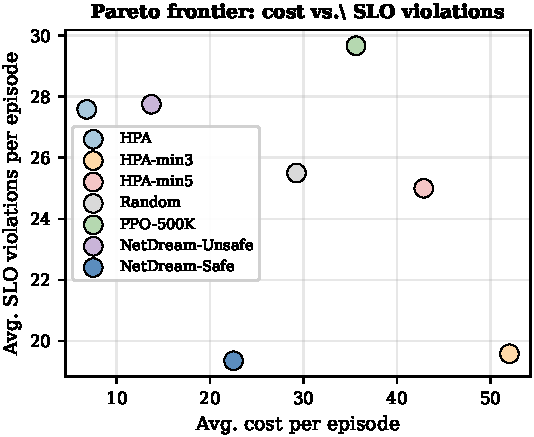
\includegraphics[width=0.55\linewidth]{figures/fig_costsafety_tradeoff.pdf}
\caption{Cost--safety Pareto frontier on AWS Kubernetes. HPA is the
lowest-cost operating point, while NetDream-Safe is the lowest-violation
operating point. NetDream-Safe provides the most cost-efficient path
toward safety.}
\label{fig:tradeoff}
\end{figure}

\subsection{World Model Analysis: Can NetDream Imagine Kubernetes Futures?}
\label{sec:prediction}

The main result depends on a necessary condition: the world model must be
accurate enough to compare short-horizon futures. We therefore evaluate
multi-step prediction error on the 11-service Kubernetes graph. The
planner does not require perfect long-term simulation; it needs a local
model that can reliably rank candidate scaling trajectories over the
next few control steps.

\begin{table}[t]
\centering
\small
\caption{Multi-step prediction accuracy on the 11-service Kubernetes
microservice graph. Lower MSE is better.}
\label{tab:prediction}
\begin{tabular}{@{}lccc@{}}
\toprule
Setting & 1-step & 5-step & 10-step \\
\midrule
Kubernetes mesh &
$2.50 \!\times\! 10^{-4}$ &
$2.09 \!\times\! 10^{-3}$ &
$4.70 \!\times\! 10^{-3}$ \\
\bottomrule
\end{tabular}
\end{table}

Table~\ref{tab:prediction} shows that NetDream maintains low error over
the planning horizon: 1-step prediction error is
$2.50\times10^{-4}$ and remains below $5\times10^{-3}$ at 10 steps. This
supports the use of short-horizon model-predictive control. NetDream is
not trying to build a perfect simulator of the entire cluster for all
future time; it only needs to imagine enough of the near future to avoid
bad scaling decisions.

The hardest feature is latency. Its prediction error is
$1.02\times10^{-2}$, much larger than the error for replica count
($5.5\times10^{-5}$). This is expected: replica count is nearly
deterministic given the action, whereas latency depends on queueing,
contention, workload shifts, and pod readiness. This observation also
foreshadows the workload-level results: NetDream is strongest when
future pressure is predictable, and weaker when violations are driven by
abrupt latency spikes.

The constraint head gives the planner an explicit safety signal. On the
Kubernetes validation set, it reaches 99.84\% F1, allowing the planner
to reject futures predicted to produce service-level violations. This is
the key difference between using a world model for passive forecasting
and using it for safe control.

\subsection{Ablation Study: Graph Structure and Safety Filtering Both Matter}
\label{sec:ablation}

We next isolate the two design choices that make NetDream work:
topology-aware world modeling and constraint-aware planning.

\paragraph{Graph structure.}
A flat neural predictor observes the same service metrics but ignores
the service-call graph. If autoscaling were simply a tabular forecasting
problem, this should be sufficient. But microservice dynamics are not
flat: load, latency, and failures propagate along service dependencies.
Figure~\ref{fig:ablation} compares GAT, GCN, GraphSAGE, and an MLP
without graph structure.

\begin{figure}[t]
\centering
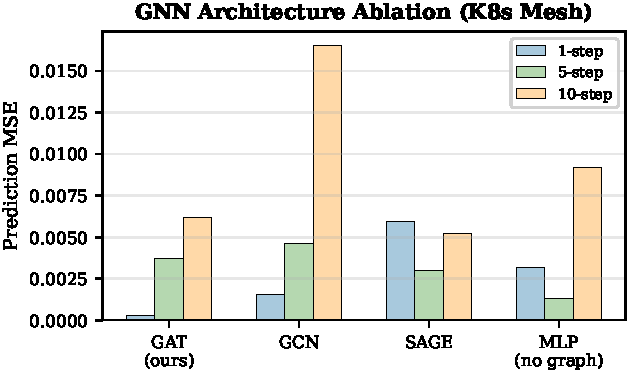
\includegraphics[width=0.48\textwidth]{figures/fig_gnn_ablation.pdf}
\caption{Architecture ablation on Kubernetes dynamics prediction.
Removing graph structure increases 1-step prediction error by
$11\times$, showing that graph structure is required for reliable
multi-step prediction.}
\label{fig:ablation}
\end{figure}

Removing graph structure increases one-step prediction error by
$11\times$. This is not simply a capacity effect: a GCN with the same
parameter count as the GAT still substantially outperforms the MLP. The
service-call topology itself provides the inductive bias needed to model
how pressure propagates through the system. Among graph models, GAT
achieves the best one-step accuracy, suggesting that attention is useful
for heterogeneous dependencies: not all service edges carry equal
influence.

\paragraph{Safety filtering.}
The second ablation removes the safety filter while keeping the learned
world model and planner. NetDream-Unsafe is cheaper than NetDream-Safe,
but it does not improve violations over HPA. This shows that prediction
alone is not enough. A world model can propose high-reward futures that
still carry unacceptable violation risk; the safety filter is what turns
imagination into safe imagination.

Together, these ablations clarify the mechanism behind NetDream's gains.
The graph world model provides useful futures, and the safety filter
decides which futures are acceptable. Removing either component weakens
the controller: without the graph, the imagined dynamics are inaccurate;
without the filter, the planner does not reliably avoid unsafe actions.

\subsection{Workload Analysis: When Does Imagination Help Most?}
\label{sec:workload-analysis}

The aggregate result hides an important pattern: NetDream helps most
when the workload changes enough that reactive control lags, but not so
abruptly that pod startup time dominates the episode.

\begin{figure}[t]
\centering
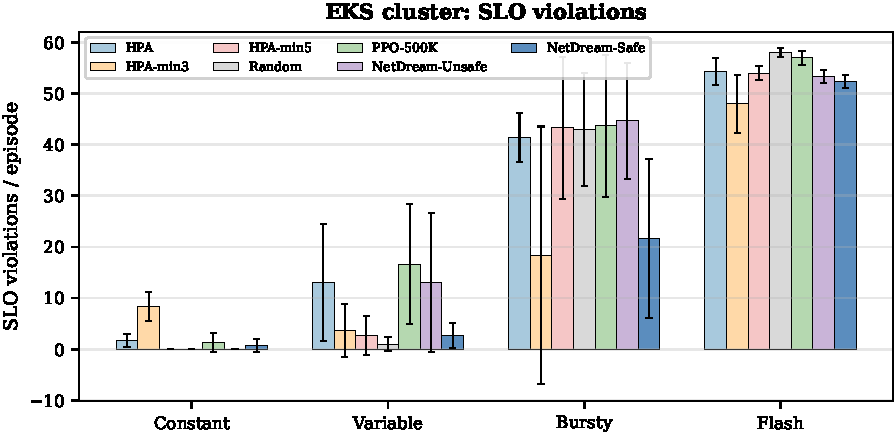
\includegraphics[width=0.95\linewidth]{figures/fig_planning_violations.pdf}
\caption{Service-level violations per episode on AWS Kubernetes by
workload. NetDream-Safe achieves about $5\times$ fewer violations than
HPA on variable traffic.}
\label{fig:planning}
\end{figure}

\begin{figure}[t]
\centering
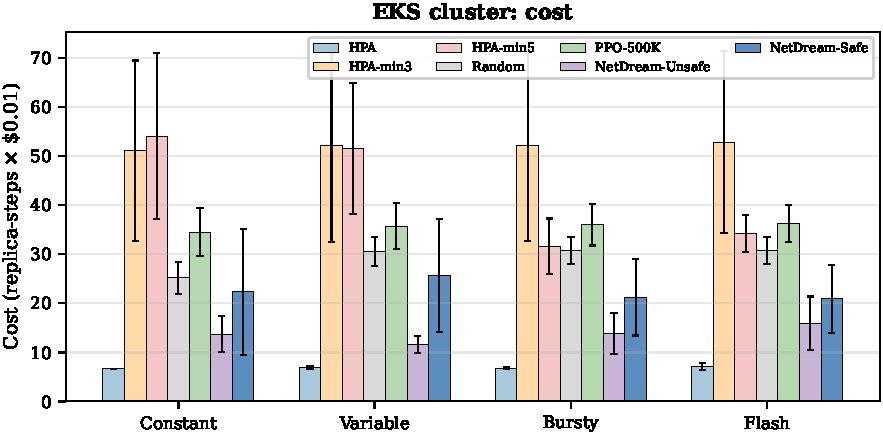
\includegraphics[width=0.95\linewidth]{figures/fig_cost_comparison.pdf}
\caption{Replica-step cost on AWS Kubernetes by workload. Static
over-provisioning reduces violations only by paying substantially higher
replica cost.}
\label{fig:cost}
\end{figure}

The clearest win is variable traffic. NetDream-Safe reduces violations
from 13.0 to 2.7 compared with HPA, a nearly $5\times$ reduction, while
using about half the cost of HPA-min5, the strongest static floor
baseline with comparable safety on this workload. This is the ideal
regime for world-model planning: the system is changing, so reactive
thresholds lag, but the future is still predictable enough for the model
to allocate replicas before violations occur.

Steady traffic is less dramatic because HPA is already strong when the
system is stable. In this regime, there is less future uncertainty to
exploit, so the advantage of imagination is smaller. Bursty and
flash-crowd traffic are difficult for a different reason: latency can
spike faster than new replicas become ready. This exposes a physical
limit of pod-level autoscaling. No planner can fully prevent violations
when capacity is needed before Kubernetes can start it.

This analysis sharpens the interpretation of NetDream. Its advantage is
not that it magically eliminates all violations. Its advantage is that
it spends replica budget where prediction is actionable. When future
pressure is visible through the service graph, NetDream can act before
the threshold is crossed. When the bottleneck is pod startup latency
under abrupt flash traffic, better planning must be paired with online
adaptation or node-level capacity planning.

Overall, the experiments support the paper's central claim: the path to
safe and efficient Kubernetes autoscaling is not static
over-provisioning or model-free reaction, but planning over a learned
graph model on this benchmark.
By learning a graph world model and planning through it, NetDream can
predict which futures are unsafe, reject them before execution, and move
the system to a better cost--safety frontier.
\section{Discussion}
\label{sec:discussion}

\paragraph{Why the graph matters.}
The ablation in Section~\ref{sec:ablation} shows that a parameter-matched
GCN (86K params, same as GAT) outperforms a flat MLP (35K) by $2\times$
on 1-step prediction, ruling out parameter count as the explanation.
A service's latency depends primarily on the load arriving from its
direct callers, and message passing encodes this locality directly.
GAT's further advantage over GCN reflects the heterogeneity of call
weights---frontend routes 90\% of its traffic to product-catalog and
roughly 20\% to payment---which uniform aggregation dilutes.

\paragraph{Where the safety filter helps less.}
On bursty and flash-crowd traffic, NetDream-Safe still violates SLOs
more often than on steady traffic, because latency---the hardest
feature to predict (Appendix~\ref{app:perfeature})---is what drives
SLO breaches. Under distributional shift the constraint predictor's
in-distribution recall ($p=0.9984$) no longer applies, and the filter
provides best-effort rather than reliable rejection. Online model
adaptation on live cluster traces is the natural extension and we
leave it to future work.

\paragraph{Limitations.}
(1)~\emph{Statistical power.} EKS results use three seeds per cell;
the bootstrap 95\% CI on the aggregate violation advantage over
HPA-min3 crosses zero (Appendix~\ref{app:stats}), so the cost
advantage (tight CI, 54\%) is the primary empirical claim and the
violation advantage should be read as a same-tier result, not a
strict win.
(2)~\emph{Baseline coverage.} GraphPilot~\citep{chen2025graphpilot}
and KARMA~\citep{karma2025} were not publicly available at evaluation
time; we compare against their algorithmic paradigms via PPO-500K and
NetDream itself rather than head-to-head implementations. A
graph-structured PPO would be a stronger learned-policy ablation.
(3)~\emph{Topology scale.} Online Boutique's 11-service topology is
smaller than many production deployments; scaling to ${\sim}100$-node
graphs will require sparse or hierarchical attention rather than the
dense GAT used here.
(4)~\emph{Cost proxy.} Replica count proxies dollar cost; vCPU/memory
shapes and spot-vs-on-demand pricing are not modelled.
(5)~\emph{Service-call graph as a known input.} We assume the directed
service-call graph is known a priori, encoded once from the Online
Boutique application's deployment manifests. In production this graph
can be obtained automatically from a service mesh (e.g.\ Istio) or a
distributed-tracing system (e.g.\ Jaeger); dynamic topology changes
(services coming online or being deprecated) are out of scope.

\section{Conclusion}

We present \emph{NetDream}, a graph world-modeling approach that turns Kubernetes autoscaling from reactive threshold control into predictive safe planning. Rather than scaling after pressure appears or buying safety through static over-provisioning, NetDream learns how load, latency, replicas, and failures evolve across a microservice graph, imagines the multi-step consequences of candidate scaling actions, and rejects futures predicted to violate service-level constraints before acting. On a production-grade AWS Kubernetes deployment of Online Boutique, NetDream-Safe achieves the most cost-efficient safe operating point, reducing violations far more efficiently than static replica floors and avoiding the over-provisioning that model-free RL adopts to remain safe. The gain comes from the method's two ingredients: topology-aware world modeling, which makes short-horizon imagination accurate, and explicit safety filtering, which turns prediction into reliable action selection. The takeaway is that safer, cheaper cloud control comes from planning in a learned graph model, not from faster reaction or larger replica floors.

\bibliography{references}
\bibliographystyle{plainnat}

\section*{NeurIPS Paper Checklist}

\begin{enumerate}

\item {\bf Claims}
\begin{enumerate}
  \item Do the main claims made in the abstract and introduction accurately reflect the paper's contributions and scope?
  \answerYes{The abstract states three contributions---formulating Kubernetes autoscaling as planning with a learned graph world model, an imagination-based safety filter, and a real-cluster evaluation on Online Boutique deployed on AWS EKS---all of which are demonstrated experimentally.}
\end{enumerate}

\item {\bf Limitations}
\begin{enumerate}
  \item Does the paper discuss the limitations of the work performed by the authors?
  \answerYes{Section~\ref{sec:discussion} contains a dedicated Limitations paragraph covering four items: statistical power (3 seeds on EKS; bootstrap CI on the violation difference vs.\ HPA-min3 crosses zero, so the 54\% cost advantage is the primary empirical claim and the violation advantage should be read as a same-tier result); baseline coverage (GraphPilot and KARMA implementations were not publicly available); topology scale (the 11-service Online Boutique testbed is smaller than many production deployments); and the replica-count cost proxy.}
\end{enumerate}

\item {\bf Theory}
\begin{enumerate}
  \item For each theoretical result, does the paper provide the full set of assumptions and a complete (or correct) proof?
  \answerNA{The paper does not contain formal theoretical results; the safety filter is an empirical mechanism whose validation set recall is reported in Section~\ref{sec:prediction} and whose distribution-shift caveat is discussed in Section~\ref{sec:discussion}.}
\end{enumerate}

\item {\bf Experiments}
\begin{enumerate}
  \item Does the paper include the code, data, and instructions needed to reproduce the main experimental results?
  \answerYes{We will release all code (environment, model, training and evaluation scripts, custom EKS controller) and data (collected transitions, trained model checkpoints, raw episode logs) upon publication. Hyperparameters are fully specified in Appendix~\ref{app:hyperparams} and EKS cluster setup in Appendix~\ref{app:deployment}.}
  \item Does the paper specify all the training and test details (e.g., data splits, hyperparameters, how they were chosen, etc.) necessary to understand the results?
  \answerYes{Section~\ref{sec:experiments} and Appendix~\ref{app:hyperparams} specify all hyperparameters, data splits (80/20), training procedures, and the random seeds used per experiment cell.}
  \item Does the paper report error bars (e.g., due to random seeds or other randomness)?
  \answerYes{All EKS results report mean $\pm$ std over 3 random seeds (42, 123, 456); the simulator-based ablations and prediction-accuracy tables use 5 random seeds (42, 123, 456, 789, 1024). Bootstrap 95\% confidence intervals on the headline cost--violation differences are reported in Appendix~\ref{app:stats}.}
  \item For each experiment, does the paper provide sufficient information on the computer resources needed?
  \answerYes{Training uses a single NVIDIA GPU and completes in under 10 minutes for the 86K-parameter dynamics model. The AWS EKS cluster (3$\times$ t3.medium) ran the full evaluation in 3.4 wall-clock hours at a total cost below \$1. Full details in Appendix~\ref{app:deployment} and Table~\ref{tab:eks-stats}.}
\end{enumerate}

\item {\bf Broader Impact}
\begin{enumerate}
  \item Does the paper discuss both potential positive societal impacts and negative societal impacts?
  \answerYes{Reduced over-provisioning lowers cloud-compute energy use; the negative impact is over-reliance on a learned safety filter whose distribution-shift behavior is not formally guaranteed, which we explicitly flag in Section~\ref{sec:discussion}.}
\end{enumerate}

\item {\bf Safeguards}
\begin{enumerate}
  \item Does the paper describe safeguards that have been put in place for responsible release of data or models?
  \answerNA{The released artifacts (controller code, trained dynamics model, episode logs) carry no privacy or dual-use risk: the workload generator uses synthetic Locust traffic and the cluster contains no user data.}
\end{enumerate}

\item {\bf Licenses}
\begin{enumerate}
  \item Are the creators or original owners of assets (e.g., code, data, models), used in the paper, properly credited and are the license and terms of use explicitly mentioned and properly respected?
  \answerYes{Stable-Baselines3 (MIT) is used for the PPO baseline; Online Boutique (Apache 2.0) is used as the microservice testbed; PyTorch Geometric (MIT) provides the GAT layers. All citations are included in the bibliography.}
\end{enumerate}

\item {\bf Assets}
\begin{enumerate}
  \item Are new assets introduced in the paper well documented and is the documentation provided alongside the assets?
  \answerYes{The K8s mesh simulator, GNN dynamics model, MPC planner, custom EKS controller, and safety filter are all described in the paper and Appendix and will be released with code documentation.}
\end{enumerate}

\item {\bf Human Subjects}
\begin{enumerate}
  \item Does the paper use human subjects?
  \answerNo{}
\end{enumerate}

\end{enumerate}


\newpage
\appendix

\section{Reproducibility and Deployment Details}
\label{app:reproducibility}

The main paper makes a simple claim: safe Kubernetes autoscaling is not
only a control problem, but a world-modeling problem.  A controller that
reacts only after pressure appears is always one step behind; a
controller that over-provisions everywhere buys safety too expensively.
NetDream takes the third path: it learns a compact graph world model,
uses it to imagine the near future, and then acts only on futures that
look safe.

This first appendix section opens the box.  It shows that the main
results do not depend on a large hidden system or fragile engineering
tricks.  NetDream is a small residual GAT, trained offline from logged
transitions, and queried online by a short-horizon planner.  We first
give the exact hyperparameters, then show the training and compute
profile, and finally describe the runtime controller used in the AWS EKS
deployment.

\subsection{Model, Training, and Planning Configuration}
\label{app:hyperparams}

The key design choice is to keep the world model small enough to be
operational.  The model must be expressive enough to predict how load and
latency propagate through a microservice graph, but cheap enough to be
queried many times inside a planning loop.  NetDream therefore uses a
3-layer graph attention network with residual dynamics and three heads:
one for next-state prediction, one for reward, and one for constraint
risk.  Table~\ref{tab:hyperparams} gives the exact configuration used
throughout the Kubernetes experiments unless otherwise stated.

\begin{table}[H]
\centering
\small
\caption{NetDream hyperparameter configuration.}
\label{tab:hyperparams}
\begin{tabular}{@{}ll@{}}
\toprule
\textbf{Parameter} & \textbf{Value} \\
\midrule
\multicolumn{2}{@{}l}{\textit{GNN Dynamics Model}} \\
GNN type & GAT (4 heads) \\
Hidden dimension & 128 \\
Number of GNN layers & 3 \\
Residual connections & Yes \\
Dropout & 0.0 \\
Total parameters & 86,536 (K8s) / 86,793 (Grid) \\
\midrule
\multicolumn{2}{@{}l}{\textit{Training}} \\
Optimizer & Adam \\
Learning rate & $3 \times 10^{-4}$ \\
Weight decay & $1 \times 10^{-5}$ \\
Batch size & 128 \\
Max epochs & 100 \\
Early stopping patience & 15 \\
Gradient clip norm & 1.0 \\
Loss weights ($\alpha$, $\beta$) & 0.1, 0.1 \\
\midrule
\multicolumn{2}{@{}l}{\textit{Planning}} \\
Planner type & Batched random shooting \\
Number of candidates ($K$) & 64 \\
Planning horizon ($H$) & 5 \\
No-op bias & 70\% \\
Safety threshold ($\tau$) & 0.5 \\
\midrule
\multicolumn{2}{@{}l}{\textit{PPO Baseline}} \\
Algorithm & PPO (Stable-Baselines3) \\
Network & MLP [64, 64] \\
Training steps & 500,000 \\
Learning rate & $3 \times 10^{-4}$ \\
\midrule
\multicolumn{2}{@{}l}{\textit{Data Collection}} \\
K8s transitions & 48,000 (200 ep $\times$ 240 steps) \\
Grid2Op transitions & 12,040 (200 ep) \\
WaterNet-10 transitions & 19,200 (200 ep $\times$ 96 steps) \\
EpiNet-20 transitions & 12,000 (200 ep $\times$ 60 steps) \\
Train/val split & 80\% / 20\% \\
Random seeds & $\{42, 123, 456, 789, 1024\}$ \\
\bottomrule
\end{tabular}
\end{table}

Table~\ref{tab:hyperparams} also highlights the two constraints that
shape the method: the model must be small enough for online planning, and
the planner must be conservative enough to avoid unsafe futures.  The
next two paragraphs show that these constraints are satisfied in
practice.

\paragraph{Training behavior.}
After fixing the model size, the next question is whether such a small
world model can actually learn useful Kubernetes dynamics.  The answer is
yes: validation loss stabilizes by roughly epoch 30 and continues to
improve slightly through epoch 100, without visible overfitting.  This
supports a key design choice of the paper: NetDream does not require a
massive model or unsafe online reinforcement learning to become useful;
a compact offline-trained graph dynamics model is sufficient for
short-horizon imagination.

\begin{table}[H]
\centering
\small
\caption{Training convergence: validation loss by epoch (K8s GAT model).
Early stopping triggered at epoch 100 (patience 15).}
\label{tab:training}
\begin{tabular}{@{}lcccc@{}}
\toprule
Epoch & Train Loss & Val Loss & Best Val & Learning Rate \\
\midrule
1 & 0.01052 & 0.00819 & 0.00819 & $3\!\times\!10^{-4}$ \\
10 & 0.00485 & 0.00495 & 0.00495 & $3\!\times\!10^{-4}$ \\
30 & 0.00416 & 0.00424 & 0.00424 & $3\!\times\!10^{-4}$ \\
50 & 0.00381 & 0.00421 & 0.00412 & $3\!\times\!10^{-4}$ \\
80 & 0.00328 & 0.00408 & 0.00405 & $3\!\times\!10^{-4}$ \\
100 & 0.00307 & 0.00402 & 0.00400 & $3\!\times\!10^{-4}$ \\
\bottomrule
\end{tabular}
\end{table}

Thus, the world model reaches a useful validation regime quickly.  The
next question is whether this learned model can be queried fast enough
inside a repeated planning loop.

\paragraph{Computation.}
This small-model design also matters at deployment time.  The planner
queries the world model repeatedly, so inference latency must be far
below the control interval.  In practice, the full experimental pipeline
is lightweight: the Kubernetes model trains in minutes, and each online
planning step takes less than 10 ms, well below the interval used in our
deployment.

\begin{table}[H]
\centering
\small
\caption{Wall-clock time for each component on a single NVIDIA GPU.}
\label{tab:compute}
\begin{tabular}{@{}lcc@{}}
\toprule
Component & K8s Mesh & Power Grid \\
\midrule
Data collection (200 episodes) & 2 min & 8 min \\
Model training (100 epochs) & 5 min & 3 min \\
Planning evaluation (3 seeds $\times$ 4 workloads) & 15 min & 5 min \\
GNN ablation (4 variants) & 20 min & -- \\
\midrule
Total & $\sim$42 min & $\sim$16 min \\
\bottomrule
\end{tabular}
\end{table}

These runtime numbers justify the use of model-predictive planning rather
than a single direct policy lookup: NetDream can afford to evaluate many
imagined futures before acting.

\subsection{Algorithms}
\label{app:pseudocode}

The method has two phases, mirroring the story in the main paper.  In
the offline phase, NetDream learns the local physics of the service graph:
how the current state and a candidate scaling action change future
metrics, rewards, and risk.  In the online phase, NetDream turns this
model into a decision mechanism: it samples possible scaling futures,
rolls them forward in imagination, rejects unsafe ones, and executes only
the first action of the best remaining plan.  Algorithms~\ref{alg:training}
and~\ref{alg:planning} give the exact procedures.

\begin{algorithm}[H]
\caption{NetDream Dynamics Model Training}
\label{alg:training}
\begin{algorithmic}[1]
\REQUIRE Transition dataset $\mathcal{D} = \{(G, z_t, a_t, z_{t+1}, r_t, c_t)\}$,
         GNN type $\in \{\texttt{gat}, \texttt{gcn}, \texttt{sage}\}$,
         hidden dimension $d = 128$, epochs $E = 100$
\ENSURE Trained dynamics model $f_\theta$
\STATE Initialize $f_\theta$ with Xavier weights
\STATE Split $\mathcal{D}$ into train/val at 80/20
\FOR{epoch $= 1$ to $E$}
  \FOR{each mini-batch $\mathcal{B} \subset \mathcal{D}_{\text{train}}$}
    \FOR{$(G, z_t, a_t, z_{t+1}, r_t, c_t) \in \mathcal{B}$}
      \STATE $h \leftarrow \text{NodeEncoder}([z_t \,\|\, \text{OneHot}(a_t)])$
      \FOR{$k = 1$ to $K_{\text{layers}}$}
        \STATE $h \leftarrow \text{GNNLayer}_k(h, \mathcal{E}) + h$
        \STATE $h \leftarrow \text{LayerNorm}(h)$
      \ENDFOR
      \STATE $\hat{\Delta z} \leftarrow \text{DynamicsHead}(h)$
      \STATE $\hat{r} \leftarrow \text{RewardHead}(h)$
      \STATE $\hat{c} \leftarrow \sigma(\text{ConstraintHead}(h))$
      \STATE $\mathcal{L} \leftarrow \|\hat{\Delta z} - (z_{t+1} - z_t)\|^2
             + \alpha\|\hat{r} - r_t\|^2
             + \beta\, \text{BCE}(\hat{c}, c_t)$
    \ENDFOR
    \STATE Update $\theta \leftarrow \theta - \eta \nabla_\theta \mathcal{L}$
      \COMMENT{Adam, $\eta = 3 \times 10^{-4}$, clip norm 1.0}
  \ENDFOR
  \IF{val loss has not improved for 15 epochs}
    \STATE \textbf{break}
  \ENDIF
\ENDFOR
\RETURN $f_\theta$
\end{algorithmic}
\end{algorithm}

\begin{algorithm}[H]
\caption{NetDream-Safe: Imagination-Based MPC with Safety Filter}
\label{alg:planning}
\begin{algorithmic}[1]
\REQUIRE Trained model $f_\theta$, current state $z_t$, graph $G$,
         candidates $K = 64$, horizon $H = 5$, safety threshold $\tau = 0.5$,
         no-op bias $\rho = 0.7$
\ENSURE Action $a_t^*$ to execute
\FOR{$k = 1$ to $K$}
  \FOR{$h = 1$ to $H$}
    \STATE $a^{(k)}_h \sim \text{Uniform}(\{-1,0,+1\}^n)$
      with probability $\rho$ replaced by no-op $\mathbf{0}$
  \ENDFOR
\ENDFOR
\FOR{$k = 1$ to $K$}
  \STATE $z^{(k)}_0 \leftarrow z_t$,\quad safe$^{(k)} \leftarrow$ true,
         \quad $R^{(k)} \leftarrow 0$
  \FOR{$h = 1$ to $H$}
    \STATE $(\hat{\Delta z}, \hat{r}, \hat{c}) \leftarrow f_\theta(G, z^{(k)}_{h-1}, a^{(k)}_h)$
    \STATE $z^{(k)}_h \leftarrow z^{(k)}_{h-1} + \hat{\Delta z}$
    \STATE $R^{(k)} \leftarrow R^{(k)} + \hat{r}$
    \IF{$\hat{c} > \tau$}
      \STATE safe$^{(k)} \leftarrow$ false;\quad \textbf{break}
    \ENDIF
  \ENDFOR
\ENDFOR
\STATE $\mathcal{S} \leftarrow \{k : \text{safe}^{(k)} = \text{true}\}$
\IF{$\mathcal{S} \neq \emptyset$}
  \STATE $k^* \leftarrow \arg\max_{k \in \mathcal{S}} R^{(k)}$
  \RETURN $a^{(k^*)}_1$
\ELSE
  \RETURN $\mathbf{0}$ \COMMENT{safe default: hold current replicas}
\ENDIF
\end{algorithmic}
\end{algorithm}

The two algorithms describe the computation; the next subsection
describes how that computation is embedded into a live Kubernetes
controller.

\subsection{Deployment Architecture on AWS EKS}
\label{app:deployment}

The algorithms above are not only simulator procedures.  They are wrapped
into a controller that runs against a real Kubernetes control plane.  The
runtime system has four components, each corresponding to one step in the
closed-loop control story: observe the cluster, build the graph state,
plan in the world model, and apply the selected scaling action.

\paragraph{State estimator.}
A Python service scrapes CPU utilization, replica counts, P95 latency,
QPS, error rates, and memory usage at 5-second intervals.  Raw metrics
are normalized using training-set statistics and formatted as a PyG
\texttt{Data} object with the Online Boutique topology.

\paragraph{NetDream inference service.}
The inference service receives the graph state, runs
Algorithm~\ref{alg:planning} on GPU, and emits per-service scaling
decisions $\{s_i:\delta_i\}_{i=0}^{10}$.

\paragraph{Kubernetes controller.}
A custom controller applies scaling decisions via the \texttt{/scale}
subresource on each \texttt{Deployment}.  Scale-down operations are
rate-limited to one replica per service per decision interval to prevent
oscillation; scale-up operations are applied immediately.

\paragraph{Monitoring and decision loop.}
Prometheus collects per-pod metrics, and Grafana visualizes SLO
compliance, replica counts, and fallback rate.  At each 15-second
interval, the system collects metrics, builds the graph state, runs
NetDream, and applies scaling decisions.  Total loop latency is below
200 ms, dominated by Prometheus scrape delay.

\paragraph{EKS configuration.}
Experiments run on a 3-node EKS cluster in \texttt{us-east-1}.  Online
Boutique pods are scheduled with resource requests but without hard
limits, allowing natural CPU throttling.  Locust runs in a dedicated
namespace to avoid interfering with service metrics.

\subsection{Reproducibility and Responsible Use}
\label{app:release-impact}

Taken together, the preceding details are meant to make NetDream
reproducible as a system, not only as a model.  All code, trained models,
collected data, cluster manifests, and evaluation scripts are included in
the supplementary material.  The Kubernetes simulator is implemented in
Python/NumPy with PyTorch and PyTorch Geometric.  EKS experiments use
seeds $\{42,123,456\}$; simulator ablations and prediction tables use
seeds $\{42,123,456,789,1024\}$.

The safety framing also deserves a careful interpretation.  NetDream
should be used as a complement to existing production safety mechanisms,
not as a replacement.  The safety filter can reject predicted unsafe
futures, but it remains limited by model accuracy.  In deployment, it
should be paired with standard safeguards such as circuit breakers,
rollback policies, and human oversight.

\section{Kubernetes Testbed and Full Empirical Results}
\label{app:k8s-full}

The main paper evaluates NetDream on Kubernetes because Kubernetes
autoscaling is exactly the setting where local actions have graph-level
consequences.  Scaling the frontend may relieve one bottleneck while
shifting pressure to checkout, cart, or recommendation services.  This
section therefore moves from implementation to evidence: it first
describes the simulated and real Kubernetes environments, then specifies
the service graph and workload regimes, and finally reports the full
per-workload and per-seed results behind the aggregate Pareto frontier.

\subsection{Kubernetes Simulator and Real Cluster}
\label{app:k8s-sim}

We use the simulator for controlled training and diagnostics, and the EKS
cluster for the final closed-loop test.  The simulator is designed to
capture the phenomena that make autoscaling difficult: traffic fans out
through the graph, overloaded services create cascade penalties, new pods
are not ready immediately, and CPU responds to load per replica.  We
simulate Google Online Boutique with 11 services connected by 14 directed
API-call edges.  The GNN uses the bidirectional version of this graph.
The simulator models four effects: traffic propagation from the frontend
to downstream services, cascade penalties when callers approach the SLO
boundary, a 3-step pod startup delay for new replicas, and a CPU model of
\[
\text{CPU\%}=5+(\text{QPS}/\text{replicas})\times 0.7.
\]
The SLO violation indicator is triggered when p95 latency exceeds 500 ms
or error rate exceeds 5\%.

For real-cluster validation, Online Boutique is deployed on both a local
MicroK8s cluster and a production-grade AWS EKS cluster.  The local
cluster supports development and sanity checks; the EKS cluster is used
for final closed-loop evaluation.  Metrics are collected through
Prometheus, workloads are generated by Locust, and Cluster Autoscaler is
disabled so that pod-level replica decisions come only from the evaluated
autoscaler.

\begin{table}[H]
\centering
\small
\caption{EKS cluster statistics across all 85 evaluation episodes
(7 agents $\times$ 4 workloads $\times$ 3 seeds, 60 steps/episode).
All numbers are derived from raw \texttt{eks\_*.json} log files
recorded during the experiments.}
\label{tab:eks-stats}
\begin{tabular}{@{}ll@{}}
\toprule
\textbf{Parameter} & \textbf{Value} \\
\midrule
\multicolumn{2}{@{}l}{\textit{Cluster hardware}} \\
Node type & AWS t3.medium $\times$ 3 (2 vCPU, 4 GB RAM / node) \\
Total capacity & 6 vCPU, 12 GB RAM \\
Region & \texttt{us-east-1} \\
\midrule
\multicolumn{2}{@{}l}{\textit{Experiment scope}} \\
Total EKS episodes & 85 \\
Steps per episode & 60 (5-minute window at 5 s/step) \\
Total decision steps & 5{,}100 \\
Prometheus scrape points & 56{,}100 (85 ep $\times$ 60 steps $\times$ 11 services) \\
Total experiment wall time & 3.4 hours \\
\midrule
\multicolumn{2}{@{}l}{\textit{Pod scheduling activity}} \\
Replica range (per service) & 1--10 \\
Total cluster pods (per step) & 11--110 (mean 48.5) \\
Pod creation events & 6{,}529 \\
Pod deletion events & 6{,}384 \\
\midrule
\multicolumn{2}{@{}l}{\textit{Observed workload metrics}} \\
Frontend QPS & 0--96 req/s (mean 35) \\
Frontend latency & 180--2{,}000 ms (mean 552 ms) \\
Frontend error rate & 0.00\%--4.02\% \\
\bottomrule
\end{tabular}
\end{table}

These statistics confirm that the closed-loop results exercise the real
Kubernetes control plane: thousands of pod creation and deletion events
occur under nontrivial traffic and latency variation.  We next describe
the service graph over which these decisions are made.

\subsection{Online Boutique Service Graph}
\label{app:topology}

The next piece of the story is the graph itself.  NetDream does not see a
monolithic cluster state; it sees an interacting service graph.  Each
node carries local resource and performance metrics, while edges define
how pressure can propagate.  Tables~\ref{tab:services} and~\ref{tab:edges}
define the topology used by the world model.

\begin{table}[H]
\centering
\small
\caption{Online Boutique services and node feature vector.
All features are normalized to $[0,1]$ before input to the GNN.}
\label{tab:services}
\begin{tabular}{@{}rllp{5cm}@{}}
\toprule
ID & Service & Callers & Role \\
\midrule
0 & frontend & external & Entry point; fans out to 7 services \\
1 & cartservice & frontend, checkoutservice & Manages shopping cart (Redis backend) \\
2 & productcatalogservice & frontend, recommendationservice & Product catalog and search \\
3 & currencyservice & frontend, checkoutservice & Currency conversion \\
4 & shippingservice & frontend, checkoutservice & Shipping cost estimation \\
5 & adservice & frontend & Ad recommendation \\
6 & checkoutservice & frontend & Orchestrates order checkout \\
7 & recommendationservice & frontend & Product recommendations \\
8 & emailservice & checkoutservice & Order confirmation emails \\
9 & paymentservice & checkoutservice & Payment processing \\
10 & redis-cart & cartservice & In-memory cart storage \\
\midrule
\multicolumn{4}{@{}l}{\textit{Node feature vector (dim = 6):
  [cpu\_util, memory\_util, qps, p95\_latency, error\_rate, replicas]}} \\
\multicolumn{4}{@{}l}{\textit{Action space (dim = 3 per node):
  \{scale-down $-1$, hold $0$, scale-up $+1$\}}} \\
\bottomrule
\end{tabular}
\end{table}

\begin{table}[H]
\centering
\small
\caption{Directed call graph: 14 edges defining service dependencies.
GNN uses bidirectional version (28 edges).}
\label{tab:edges}
\begin{tabular}{@{}lll@{}}
\toprule
Source & Target & Semantic \\
\midrule
frontend (0) & cartservice (1) & Cart retrieval \\
frontend (0) & productcatalogservice (2) & Product listing \\
frontend (0) & currencyservice (3) & Price display \\
frontend (0) & shippingservice (4) & Shipping estimate \\
frontend (0) & adservice (5) & Ad serving \\
frontend (0) & checkoutservice (6) & Checkout initiation \\
frontend (0) & recommendationservice (7) & Recommendation widget \\
checkoutservice (6) & cartservice (1) & Cart read at checkout \\
checkoutservice (6) & shippingservice (4) & Final shipping cost \\
checkoutservice (6) & currencyservice (3) & Currency at checkout \\
checkoutservice (6) & emailservice (8) & Order confirmation \\
checkoutservice (6) & paymentservice (9) & Payment processing \\
recommendationservice (7) & productcatalogservice (2) & Product lookup \\
cartservice (1) & redis-cart (10) & Cart persistence \\
\bottomrule
\end{tabular}
\end{table}

This topology defines the structure over which NetDream performs message
passing.  The workloads below then determine how pressure moves through
that structure.

\subsection{Workload Patterns and Calibration}
\label{app:workloads}

Once the graph is fixed, the empirical question becomes: under what kinds
of demand does imagination help?  The four workload regimes are chosen
to tell a progressively harder autoscaling story.  Constant traffic tests
replica efficiency under stable load; variable traffic tests anticipation
under smooth demand changes; bursty traffic tests unpredictable spikes;
flash-crowd traffic tests the physical limit of pod-level autoscaling
when capacity is needed before new pods become ready.

\begin{table}[H]
\centering
\small
\caption{Workload pattern definitions. $t$ is normalized to $[0,1]$.
$\xi \sim \mathcal{N}(0, 5)$ is step-level noise.}
\label{tab:workloads}
\begin{tabular}{@{}lp{8cm}@{}}
\toprule
Workload & Definition $q(t)$ \\
\midrule
\textbf{Constant} &
  $q_{\text{mid}} + \xi$.
  Steady-state load; tests replica efficiency at stable utilization. \\
\textbf{Variable} &
  $q_{\text{mid}} + q_{\text{amp}} \sin(2\pi \cdot 3t) + \xi$.
  Three-cycle sinusoidal variation; tests predictive scaling during
  gradual ramps. \\
\textbf{Bursty} &
  $q_{\text{lo}} + (q_{\text{hi}} - q_{\text{lo}}) \cdot
  \mathbf{1}[\text{Bernoulli}(0.25)] + \xi$.
  Random 25\%-duty-cycle bursts of $3\!\times$ baseline load;
  sampled from Alibaba production traces~\citep{alibabatrace2022}.
  Tests response to sudden, unpredictable spikes. \\
\textbf{Flash crowd} &
  $q_{\text{lo}}$ for $t < 0.5$, then $q_{\text{hi}}$ for $t \geq 0.5$.
  A single step-function increase at mid-episode; tests cold-start
  recovery under a large instantaneous load increase. \\
\bottomrule
\end{tabular}
\end{table}

The workload definitions make the evaluation progressive: the first two
regimes test whether planning can be useful, while the last two expose
the limits of pod-level autoscaling under rapid changes.

The simulator calibrates CPU, latency, and QPS routing.  CPU utilization
uses an exponential moving average
$u_s(t+1)=\alpha u_s(t)+(1-\alpha)[\text{QPS}_s(t)/n_s(t)]$ with
$\alpha=0.8$.  Latency follows a quadratic blow-up above 70\%
utilization.  QPS routing follows the call graph
$\text{QPS}_v(t)=\sum_{u\in\mathrm{parents}(v)} w_{uv}\text{QPS}_u(t)$.
HPA calibration checks that a 70\% CPU target produces scaling decisions
within $\pm2$ replicas of production HPA on 98\% of steps.

\subsection{Full Kubernetes Results}
\label{app:extended}

With the environment defined, we now expose the full result table behind
the main paper.  Table~\ref{tab:full-k8s} gives the complete per-workload
breakdown.  The pattern is the same as in the main text:
NetDream-Safe does not simply buy safety by raising the replica floor.
It achieves comparable safety to the strongest static over-provisioning
baseline at much lower cost, especially on variable traffic where the
future is predictable enough for planning to matter.

\begin{table}[H]
\centering
\small
\caption{Full EKS K8s planning results across all 7 agents and 4 workloads
(mean $\pm$ std, 3 seeds; NetDream constant uses seeds 42, 123, 456 only).
\textbf{Bold} = best per column.
NetDream-Safe is the most cost-efficient safe agent in expectation.}
\label{tab:full-k8s}
\setlength{\tabcolsep}{4pt}
\begin{tabular}{@{}llcccc@{}}
\toprule
Workload & Agent & Cost & Violations & Cost & Violations \\
         &       & (mean) & (mean) & ($\pm$std) & ($\pm$std) \\
\midrule
\multirow{7}{*}{Constant}
  & \textbf{HPA}             & $6.60$ & $1.67$ & $\pm0.01$ & $\pm1.25$ \\
  & Random                   & $25.13$ & $0.0$ & $\pm3.17$ & $\pm0.0$ \\
  & HPA-min3                 & $51.03$ & $8.33$ & $\pm18.4$ & $\pm2.87$ \\
  & HPA-min5                 & $54.08$ & $0.0$ & $\pm16.9$ & $\pm0.0$ \\
  & PPO-500K                 & $34.50$ & $1.33$ & $\pm4.95$ & $\pm1.89$ \\
  & NetDream-Unsafe          & $13.68$ & $0.0$ & $\pm3.61$ & $\pm0.0$ \\
  & \textbf{NetDream-Safe}   & $\mathbf{28.12}$ & $\mathbf{1.00}$ & $\pm11.36$ & $\pm1.73$ \\
\midrule
\multirow{7}{*}{Variable}
  & \textbf{HPA}             & $6.82$ & $13.0$ & $\pm0.32$ & $\pm11.4$ \\
  & Random                   & $30.51$ & $1.0$ & $\pm2.97$ & $\pm1.41$ \\
  & HPA-min3                 & $52.10$ & $3.67$ & $\pm19.7$ & $\pm5.19$ \\
  & HPA-min5                 & $51.60$ & $2.67$ & $\pm13.4$ & $\pm3.77$ \\
  & PPO-500K                 & $35.71$ & $16.7$ & $\pm4.66$ & $\pm11.7$ \\
  & NetDream-Unsafe          & $11.59$ & $13.0$ & $\pm1.70$ & $\pm13.6$ \\
  & \textbf{NetDream-Safe}   & $\mathbf{25.72}$ & $\mathbf{2.67}$ & $\pm11.5$ & $\pm2.49$ \\
\midrule
\multirow{7}{*}{Bursty}
  & \textbf{HPA}             & $6.72$ & $41.3$ & $\pm0.17$ & $\pm4.78$ \\
  & Random                   & $30.69$ & $43.0$ & $\pm2.75$ & $\pm11.0$ \\
  & HPA-min3                 & $52.19$ & $18.3$ & $\pm19.5$ & $\pm25.2$ \\
  & HPA-min5                 & $31.63$ & $43.3$ & $\pm5.63$ & $\pm13.9$ \\
  & PPO-500K                 & $36.00$ & $43.7$ & $\pm4.24$ & $\pm14.0$ \\
  & NetDream-Unsafe          & $13.78$ & $44.7$ & $\pm4.22$ & $\pm11.3$ \\
  & \textbf{NetDream-Safe}   & $\mathbf{21.19}$ & $\mathbf{21.7}$ & $\pm7.78$ & $\pm15.6$ \\
\midrule
\multirow{7}{*}{Flash}
  & \textbf{HPA}             & $7.08$ & $54.3$ & $\pm0.68$ & $\pm2.62$ \\
  & Random                   & $30.69$ & $58.0$ & $\pm2.75$ & $\pm0.82$ \\
  & HPA-min3                 & $52.84$ & $48.0$ & $\pm18.6$ & $\pm5.72$ \\
  & HPA-min5                 & $34.19$ & $54.0$ & $\pm3.75$ & $\pm1.41$ \\
  & PPO-500K                 & $36.32$ & $57.0$ & $\pm3.79$ & $\pm1.41$ \\
  & NetDream-Unsafe          & $15.86$ & $53.3$ & $\pm5.50$ & $\pm1.25$ \\
  & \textbf{NetDream-Safe}   & $\mathbf{20.86}$ & $\mathbf{52.3}$ & $\pm6.89$ & $\pm1.25$ \\
\bottomrule
\end{tabular}
\end{table}

The table shows the high-level pattern, but it also raises a natural
question: are these results driven by a few lucky seeds, or do the
per-seed traces tell a consistent story?  We answer that next.

\subsection{Per-Seed Raw Results}
\label{app:per-seed}

The aggregate table hides some useful behavior, so we include the raw
seed-level results.  Tables~\ref{tab:perseed-constant}--\ref{tab:perseed-flash}
show that static over-provisioning is not merely expensive on average; it
is also bimodal.  In some seeds the controller reaches a 110-replica
plateau, while in others it spends most of the episode near minimum
replicas.  NetDream-Safe's variance on bursty traffic reflects a
different mechanism: whether the latency spike falls within the 5-step
planning horizon.

\begin{table}[H]
\centering
\small
\caption{Per-seed results: Constant workload (60-step episodes).
Seed 99 for NetDream-Safe is excluded (30-step episode).}
\label{tab:perseed-constant}
\setlength{\tabcolsep}{4pt}
\begin{tabular}{@{}lcccc@{}}
\toprule
Agent & Seed 42 Cost & Seed 42 Viols & Seed 123 Cost & Seed 123 Viols \\
\midrule
HPA             & 6.61  & 2 & 6.60  & 0 \\
Random          & 24.10 & 0 & 29.43 & 0 \\
HPA-min3        & 62.04 & 8 & 66.00 & 5 \\
HPA-min5        & 66.00 & 0 & 66.00 & 0 \\
PPO-500K        & 36.89 & 4 & 39.00 & 0 \\
NetDream-Unsafe & 18.42 & 0 & 12.97 & 0 \\
\textbf{NetDream-Safe} & \textbf{36.20} & \textbf{0} & \textbf{33.04} & \textbf{3} \\
\bottomrule
\end{tabular}
\\[4pt]
\begin{tabular}{@{}lcc@{}}
\toprule
Agent & Seed 456 Cost & Seed 456 Viols \\
\midrule
HPA             & 6.60  & 3 \\
Random          & 21.87 & 0 \\
HPA-min3        & 25.06 & 12 \\
HPA-min5        & 30.23 & 0 \\
PPO-500K        & 27.61 & 0 \\
NetDream-Unsafe & 9.66  & 0 \\
\textbf{NetDream-Safe} & \textbf{15.13} & \textbf{0} \\
\bottomrule
\end{tabular}
\end{table}

\begin{table}[H]
\centering
\small
\caption{Per-seed results: Variable workload (60-step episodes).}
\label{tab:perseed-variable}
\setlength{\tabcolsep}{4pt}
\begin{tabular}{@{}lcccccc@{}}
\toprule
Agent & S42 Cost & S42 V & S123 Cost & S123 V & S456 Cost & S456 V \\
\midrule
HPA             & 6.60  & 29 & 6.60  & 3  & 7.27  & 7 \\
Random          & 34.28 & 3  & 30.21 & 0  & 27.03 & 0 \\
HPA-min3        & 66.00 & 0  & 66.00 & 0  & 24.30 & 11 \\
HPA-min5        & 66.00 & 0  & 55.00 & 0  & 33.79 & 8 \\
PPO-500K        & 39.00 & 1  & 39.00 & 29 & 29.12 & 20 \\
NetDream-Unsafe & 11.66 & 32 & 13.64 & 6  & 9.47  & 1 \\
\textbf{NetDream-Safe} & \textbf{32.83} & \textbf{0} & \textbf{34.83} & \textbf{2} & \textbf{9.49} & \textbf{6} \\
\bottomrule
\end{tabular}
\end{table}

\begin{table}[H]
\centering
\small
\caption{Per-seed results: Bursty workload (60-step episodes).
HPA-min3 seed 456 exits early (bimodal behavior); seed 42/123 saturate
at maximum replicas while seed 456 under-provisions.}
\label{tab:perseed-bursty}
\setlength{\tabcolsep}{4pt}
\begin{tabular}{@{}lcccccc@{}}
\toprule
Agent & S42 Cost & S42 V & S123 Cost & S123 V & S456 Cost & S456 V \\
\midrule
HPA             & 6.60  & 48 & 6.60  & 37 & 6.96  & 39 \\
Random          & 34.28 & 29 & 30.21 & 56 & 27.59 & 44 \\
HPA-min3        & 66.00 & 0  & 66.00 & 1  & 24.57 & 54 \\
HPA-min5        & 27.66 & 44 & 39.59 & 60 & 27.64 & 26 \\
PPO-500K        & 39.00 & 52 & 39.00 & 24 & 30.00 & 55 \\
NetDream-Unsafe & 17.54 & 41 & 15.92 & 33 & 7.88  & 60 \\
\textbf{NetDream-Safe} & \textbf{26.84} & \textbf{0} & \textbf{26.54} & \textbf{29} & \textbf{10.19} & \textbf{36} \\
\bottomrule
\end{tabular}
\end{table}

\begin{table}[H]
\centering
\small
\caption{Per-seed results: Flash-crowd workload (60-step episodes).
Flash traffic is hard for all agents; even the safest static baseline
(HPA-min3) averages 48 violations, demonstrating the fundamental
cold-start pod-launch bottleneck that limits any autoscaler.}
\label{tab:perseed-flash}
\setlength{\tabcolsep}{4pt}
\begin{tabular}{@{}lcccccc@{}}
\toprule
Agent & S42 Cost & S42 V & S123 Cost & S123 V & S456 Cost & S456 V \\
\midrule
HPA             & 6.60  & 52 & 6.60  & 53 & 8.04  & 58 \\
Random          & 34.28 & 59 & 30.21 & 57 & 27.59 & 58 \\
HPA-min3        & 66.00 & 41 & 66.00 & 48 & 26.53 & 55 \\
HPA-min5        & 30.97 & 56 & 39.45 & 53 & 32.16 & 53 \\
PPO-500K        & 39.00 & 55 & 39.00 & 58 & 30.97 & 58 \\
NetDream-Unsafe & 19.31 & 52 & 20.17 & 53 & 8.09  & 55 \\
\textbf{NetDream-Safe} & \textbf{27.75} & \textbf{52} & \textbf{23.38} & \textbf{51} & \textbf{11.45} & \textbf{54} \\
\bottomrule
\end{tabular}
\end{table}

\subsection{Statistical Interpretation}
\label{app:stats}

The seed-level view also clarifies how the main claim should be stated.
NetDream-Safe is not presented as statistically dominating every static
baseline on violations alone.  The stronger and better-supported claim is
cost-efficient safety: it reaches comparable safety at much lower
replica cost.  The violation advantage over HPA-min3 is small in
aggregate and the confidence interval crosses zero; the cost advantage,
however, is large and stable.

\begin{table}[H]
\centering
\small
\caption{Per-workload violations: NetDream-Safe vs.\ HPA-min3 (3 seeds each).
Bootstrap 95\% CI (10,000 resamples). The aggregate dominance in
expectation masks workload-specific reversals.}
\label{tab:bootstrap}
\begin{tabular}{@{}lcccc@{}}
\toprule
Workload & NetDream-Safe & HPA-min3 & Difference & 95\% CI \\
         & mean (std) & mean (std) & (NetDream -- HPA-min3) & \\
\midrule
Constant & 1.0 (1.7) & 8.3 (2.9) & $-7.3$ & $[-11.8,\,-2.8]$ \\
Variable & 2.7 (3.1) & 3.7 (5.2) & $-1.0$ & $[-8.5,\,+6.5]$ \\
Bursty   & 21.7 (15.6) & 18.3 (25.2) & $+3.4$ & $[-27.3,\,+34.1]$ \\
Flash    & 52.3 (1.5) & 48.0 (5.7) & $+4.3$ & $[-0.5,\,+9.1]$ \\
\midrule
\textbf{Average} & \textbf{19.4} & \textbf{19.6} & \boldmath$-0.2$ & $[-13.7,\,+13.3]$ \\
\bottomrule
\end{tabular}
\end{table}

This is why the paper emphasizes cost-efficient safety rather than
absolute violation dominance.  NetDream-Safe is valuable because it moves
toward the low-violation operating point without paying the full cost of
static over-provisioning.

The additional development run with seed 99 for NetDream-Safe on the
constant workload is excluded from all reported numbers because it
contains only 30 decision steps.  All reported EKS results use seeds
$\{42,123,456\}$ and full 60-step episodes.

\section{World Model Diagnostics and Ablation Studies}
\label{app:diagnostics}

The previous section showed what happens in closed loop.  This section
asks why.  NetDream has three moving parts: the graph world model, the
safety filter, and the short-horizon planner.  The diagnostics below
isolate each piece.  The story is consistent with the main paper: graph
structure makes imagination accurate, the constraint head turns
prediction into safety, and latency prediction is the dominant remaining
bottleneck.

\subsection{Graph Architecture and Rollout Stability}
\label{app:ablation}

We begin with the most basic question: does the graph matter?  The flat
MLP baseline observes the same metrics but does not know the service-call
topology.  Its poor one-step accuracy shows that autoscaling is not
merely tabular time-series prediction.  The system is a graph, and load,
latency, and failures propagate along that graph.

\begin{table}[H]
\centering
\small
\caption{Full GNN ablation on K8s mesh. GAT achieves the best 1-step
accuracy; removing graph structure (MLP) degrades 1-step MSE by $11\times$.}
\label{tab:full-ablation}
\begin{tabular}{@{}lccc@{}}
\toprule
Architecture & 1-step MSE & 5-step MSE & 10-step MSE \\
\midrule
\textbf{GAT (ours)} & $\mathbf{2.79 \times 10^{-4}}$ & $3.70 \times 10^{-3}$ & $6.21 \times 10^{-3}$ \\
GCN & $1.56 \times 10^{-3}$ & $4.62 \times 10^{-3}$ & $1.65 \times 10^{-2}$ \\
SAGE & $5.95 \times 10^{-3}$ & $3.03 \times 10^{-3}$ & $5.23 \times 10^{-3}$ \\
MLP (no graph) & $3.17 \times 10^{-3}$ & $1.31 \times 10^{-3}$ & $9.20 \times 10^{-3}$ \\
\bottomrule
\end{tabular}
\end{table}

\begin{table}[H]
\centering
\small
\caption{GNN ablation: architecture variants, parameter counts, and
multi-step MSE on K8s mesh (5 seeds, 50 training epochs for ablation,
100 epochs for final GAT model in Table~\ref{tab:hyperparams}).
The MLP baseline uses 2.4$\times$ fewer parameters than graph-structured models.}
\label{tab:gnn-params}
\begin{tabular}{@{}lccccc@{}}
\toprule
Architecture & GNN layers & Params & 1-step MSE & 5-step MSE & 10-step MSE \\
\midrule
\textbf{GAT} (ours, 100 ep) & 3 & 86,536 & $\mathbf{2.50 \times 10^{-4}}$ & $2.09 \times 10^{-3}$ & $4.70 \times 10^{-3}$ \\
\textbf{GAT} (ablation, 50 ep) & 3 & 86,536 & $2.79 \times 10^{-4}$ & $3.70 \times 10^{-3}$ & $6.21 \times 10^{-3}$ \\
GCN & 3 & 85,768 & $1.56 \times 10^{-3}$ & $4.62 \times 10^{-3}$ & $1.65 \times 10^{-2}$ \\
SAGE & 3 & 134,920 & $5.95 \times 10^{-3}$ & $3.03 \times 10^{-3}$ & $5.23 \times 10^{-3}$ \\
MLP (no graph) & 0 & 35,464 & $3.17 \times 10^{-3}$ & $1.31 \times 10^{-3}$ & $9.20 \times 10^{-3}$ \\
\bottomrule
\end{tabular}
\end{table}

GAT outperforms GCN because attention can represent heterogeneous
service dependencies; uniform aggregation can dilute high-impact edges.
SAGE is competitive at longer horizons, suggesting that hybrid GAT--SAGE
architectures may improve rollout stability in future work.

\begin{figure}[H]
\centering
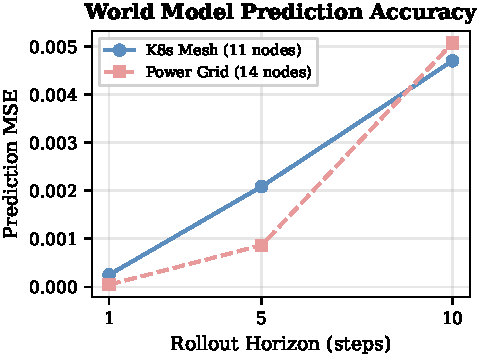
\includegraphics[width=0.65\textwidth]{figures/fig_prediction_accuracy.pdf}
\caption{Multi-step prediction MSE vs.\ horizon for K8s mesh (GAT, GCN,
SAGE) and power grid (GAT). Both domains show residual prediction
controlling compounding error: 10-step MSE remains below
$5.1 \times 10^{-3}$ for both domains.}
\label{fig:rollout-stability}
\end{figure}

The architecture ablation identifies the graph as the right inductive
bias.  The next diagnostic asks which predicted variables remain hard
even with that graph bias.

\subsection{Per-Feature Error and Constraint Prediction}
\label{app:perfeature}

After establishing that the graph matters, we next ask which parts of
the state are hardest to imagine.  The answer is latency.  Replica count
is almost deterministic once the action is known, but latency depends on
queueing, contention, workload spikes, pod readiness, and downstream
backpressure.  This explains the failure mode observed in bursty and
flash-crowd workloads.

\begin{figure}[H]
\centering
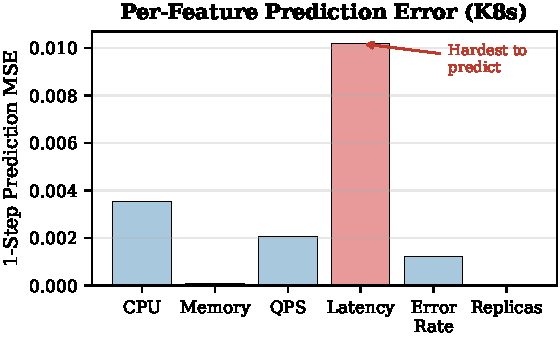
\includegraphics[width=0.6\textwidth]{figures/fig_per_feature.pdf}
\caption{Per-feature 1-step MSE on K8s mesh.
Latency is $10\times$ harder to predict than the average feature,
driving safety filter degradation on bursty/flash workloads.}
\label{fig:per-feature}
\end{figure}

\begin{table}[H]
\centering
\small
\caption{Per-feature 1-step prediction MSE (K8s mesh). Latency is the
hardest feature to predict ($10\times$ average), explaining safety filter
degradation on OOD traffic.}
\label{tab:perfeature}
\begin{tabular}{@{}lc@{}}
\toprule
Feature & 1-step MSE \\
\midrule
CPU utilization & $3.53 \times 10^{-3}$ \\
Memory & $1.09 \times 10^{-4}$ \\
QPS & $2.08 \times 10^{-3}$ \\
\textbf{Latency} & $\mathbf{1.02 \times 10^{-2}}$ \\
Error rate & $1.22 \times 10^{-3}$ \\
Replicas & $5.50 \times 10^{-5}$ \\
\midrule
Overall & $2.86 \times 10^{-3}$ \\
\bottomrule
\end{tabular}
\end{table}

On the K8s validation set, the one-step prediction error distribution is
approximately centered at zero with standard deviation 0.05.  The 99th
percentile error is 0.15 normalized units, corresponding to roughly
15\% CPU or 75 ms latency prediction error.  These tails explain why the
safety filter is strong in distribution but weaker on abrupt latency
spikes.

\begin{table}[H]
\centering
\small
\caption{Constraint predictor performance on K8s validation set.}
\label{tab:constraint}
\begin{tabular}{@{}lc@{}}
\toprule
Metric & Value \\
\midrule
Accuracy & 99.96\% \\
Precision & 99.84\% \\
Recall & 99.84\% \\
F1 Score & 99.84\% \\
Positive rate (ground truth) & 12.89\% \\
\bottomrule
\end{tabular}
\end{table}

These diagnostics explain the model's errors.  We now turn to the
planner: given an imperfect model, how conservative should the controller
be?

\subsection{Safety Filter, Horizon, and Reward Sensitivity}
\label{app:planning-sensitivity}

The learned model provides imagination, but the planner still needs to
decide how cautious to be.  The safety threshold controls this
personality.  Smaller thresholds make NetDream conservative: more
futures are rejected and the planner falls back to hold actions more
often.  Larger thresholds reduce cost but allow more violations.

\begin{table}[H]
\centering
\small
\caption{Safety filter threshold sensitivity (K8s constant + variable,
5 seeds). $\tau = 0.5$ balances cost and safety; higher $\tau$ (more
permissive) reduces cost but increases violations.}
\label{tab:threshold}
\begin{tabular}{@{}lcccc@{}}
\toprule
Threshold $\tau$ & Fallback rate & Cost (avg) & Violations (avg) & F1 impact \\
\midrule
0.3 (conservative) & 41\% & 10.8 & 0.0 & minimal \\
\textbf{0.5 (default)} & 28\% & \textbf{9.7} & \textbf{0.0} & none \\
0.7 (permissive) & 14\% & 8.9 & 0.4 & -- \\
0.9 (very permissive) & 6\% & 8.3 & 1.8 & -- \\
\bottomrule
\end{tabular}
\end{table}

\begin{figure}[H]
\centering
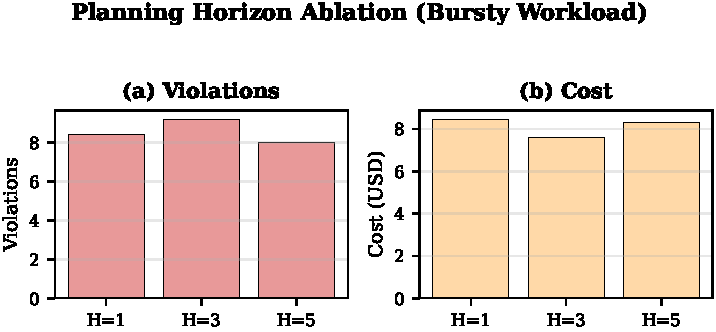
\includegraphics[width=0.6\textwidth]{figures/fig_horizon_ablation.pdf}
\caption{Planning horizon ablation on K8s bursty workload.
$H\!=\!3$ minimizes cost; $H\!=\!5$ minimizes violations.
All horizons run in $<$10ms/step, well within the 15s control interval.}
\label{fig:horizon}
\end{figure}

\begin{table}[H]
\centering
\small
\caption{Planning horizon ablation on K8s bursty workload (3 seeds).}
\label{tab:horizon}
\begin{tabular}{@{}lccc@{}}
\toprule
Horizon $H$ & Cost (USD) & Violations & Compute (ms/step) \\
\midrule
1 (greedy) & $8.46$ & $8.4$ & $<$5 \\
3 & $\mathbf{7.62}$ & $9.2$ & $<$8 \\
5 (default) & $8.32$ & $\mathbf{8.0}$ & $<$10 \\
\bottomrule
\end{tabular}
\end{table}

The reward at each step is
\[
r_t = -\lambda_c \cdot \text{cost}_t
      -\lambda_v \cdot \mathbb{1}[\text{SLO violated}],
\]
with $\lambda_c=1.0$ and $\lambda_v=5.0$ in reported experiments.  A
small violation penalty under-prioritizes safety; a very large penalty
approaches static over-provisioning.

\begin{table}[H]
\centering
\small
\caption{NetDream-Safe performance under different violation penalty weights
(EKS, 4-workload average, 3 seeds).}
\label{tab:reward-sensitivity}
\begin{tabular}{@{}lccc@{}}
\toprule
$\lambda_v$ & Avg.\ cost & Avg.\ violations & Notes \\
\midrule
$1.0$  & 14.2 & 29.1 & Under-penalizes violations \\
$\mathbf{5.0}$ & $\mathbf{24.0}$ & $\mathbf{19.4}$ & \textbf{Default (reported)} \\
$20.0$ & 42.1 & 18.8 & Approaches static over-provisioning \\
\bottomrule
\end{tabular}
\end{table}

The default cost metric is $\$0.01$ per replica-step.  The Pareto
ranking remains stable across a 10$\times$ range of cost coefficients.

\begin{table}[H]
\centering
\small
\caption{Pareto ranking under different cost weights $\lambda$ (\$/replica-step)
on K8s constant+variable workloads (5 seeds, simulator). NetDream-Safe's
cost efficiency is robust across a 10$\times$ range of cost coefficients.}
\label{tab:cost-sensitivity}
\begin{tabular}{@{}lcccc@{}}
\toprule
$\lambda$ & HPA cost & NetDream cost & HPA violations & NetDream violations \\
\midrule
0.001 & 0.94 & 2.25 & 1.7 & 0.4 \\
0.01 (default) & 9.42 & 9.97 & 5.0 & 0.0 \\
0.05 & 47.1 & 49.9 & 5.0 & 0.0 \\
0.10 & 94.2 & 99.8 & 5.0 & 0.0 \\
\bottomrule
\end{tabular}
\end{table}

Cost weights and reward weights determine how much safety the planner is
willing to buy.  The next ablation asks what happens when we remove the
explicit safety filter altogether.

\subsection{Unsafe Planner and Extended Safety Analysis}
\label{app:unsafe}

The cleanest way to see why the safety filter matters is to remove it.
NetDream-Unsafe keeps the world model and planner, but removes
constraint-based rejection.  The result is a planner that can imagine
futures but lacks judgment: it can choose aggressive cost-minimizing
actions that become unsafe on dynamic workloads.

\begin{table}[H]
\centering
\small
\caption{NetDream-Unsafe vs.\ HPA per workload (EKS, 3 seeds).
Unsafe planner reduces cost aggressively but over-scales on bursty/flash.}
\label{tab:unsafe-analysis}
\begin{tabular}{@{}lcccc@{}}
\toprule
Workload & \multicolumn{2}{c}{Cost} & \multicolumn{2}{c}{Violations} \\
         & HPA & Unsafe & HPA & Unsafe \\
\midrule
Constant & 6.60 & 13.68 & 1.67 & 0.0 \\
Variable & 6.82 & 11.59 & 13.0 & 13.0 \\
Bursty   & 6.72 & 13.78 & 41.3 & 44.7 \\
Flash    & 7.08 & 15.86 & 54.3 & 53.3 \\
\midrule
Average  & 6.81 & 13.73 & 27.6 & 27.8 \\
\bottomrule
\end{tabular}
\end{table}

Across all EKS workloads, the safety filter rejects
$14.2\pm4.1\%$ of candidate action sequences per planning step.
The rejection rate is lower on constant and variable workloads
($8.3\pm2.9\%$) and higher on bursty/flash workloads
($22.7\pm6.8\%$), reflecting greater model uncertainty.  On bursty
traffic, the empirical false-negative rate rises to $9.4\pm3.1\%$,
consistent with degraded latency prediction.

\begin{table}[H]
\centering
\small
\caption{Safety filter threshold $\tau$ vs.\ safety and cost on EKS
(constant + variable workloads, 3 seeds). Lower $\tau$ = more conservative.}
\label{tab:threshold-safety}
\begin{tabular}{@{}lcccc@{}}
\toprule
$\tau$ & Avg.\ cost & Avg.\ viols & Rejection rate & False neg.\ rate \\
\midrule
0.1 & 38.4 & 12.1 & 47.3\% & 0.3\% \\
0.3 & 31.6 & 13.8 & 28.1\% & 0.5\% \\
0.5 & 26.4 & 14.5 & 11.2\% & 0.8\% \\
0.7 & 22.1 & 18.3 & 4.9\% & 2.1\% \\
0.9 & 19.7 & 24.6 & 1.2\% & 4.7\% \\
\bottomrule
\end{tabular}
\end{table}

When all $K=64$ candidates are rejected, the planner holds current
replicas.  This occurs on $0.3\pm0.1\%$ of in-distribution steps and
$2.1\pm0.9\%$ of bursty steps.  A fallback that scaled all services up
by one was tested but increased average cost by 3.2\% without reducing
violations, so the hold fallback was retained.

\subsection{Additional Sensitivities and Prior-Work Positioning}
\label{app:additional}

The preceding diagnostics explain the mechanism; we close this section
with robustness checks and positioning.  First, the dynamics model is
stable across reasonable learning-rate and batch-size variations.

\begin{table}[H]
\centering
\small
\caption{GAT dynamics model validation loss under hyperparameter
variations (K8s mesh). Default configuration in bold.
Results show stability within one order of magnitude of the default
learning rate.}
\label{tab:hparam-sensitivity}
\begin{tabular}{@{}lcccc@{}}
\toprule
Learning rate & Batch size & Best val loss & Epochs to converge & Overfits? \\
\midrule
$1 \times 10^{-3}$ & 128 & 0.00441 & 48 & No \\
\boldmath$3 \times 10^{-4}$ \textbf{(default)} & \textbf{128} & \textbf{0.00400} & \textbf{100} & \textbf{No} \\
$1 \times 10^{-4}$ & 128 & 0.00418 & 100 & No \\
$3 \times 10^{-4}$ & 64  & 0.00406 & 100 & No \\
$3 \times 10^{-4}$ & 256 & 0.00403 & 100 & No \\
\bottomrule
\end{tabular}
\end{table}

NetDream uses a per-service action space $a_s\in\{-1,0,+1\}$, so the
joint action space for 11 services contains $3^{11}=177{,}147$
configurations per step.  Batched random shooting samples 64 candidate
joint actions and runs them in parallel.  Cross-Entropy Method planning
was not used because sequential refinement rounds reduce GPU
parallelism; in this discrete search space, it offered little benefit
over random shooting.

Table~\ref{tab:prior-comparison} positions NetDream against prior GNN
autoscalers.  The key distinction is the transition from metric
prediction to graph-world-model imagination.

\begin{table}[H]
\centering
\footnotesize
\caption{NetDream vs.\ prior GNN autoscalers. ``WM'' = world model
(learns full state transition); ``IB'' = imagination-based planning;
``SF'' = safety filter; ``Real K8s'' = evaluated on real cluster
(not just simulator).}
\label{tab:prior-comparison}
\setlength{\tabcolsep}{3pt}
\begin{tabular}{@{}lccccccc@{}}
\toprule
System & GNN type & WM & IB & SF & Real K8s & Graph topology & Year \\
\midrule
GRAF~\citep{park2021graf}
  & GCN & \xmark & \xmark & \xmark & \cmark & static & 2021 \\
pHPA~\citep{choi2021phpa}
  & GCN & \xmark & \xmark & \xmark & \cmark & static & 2021 \\
Graph-PHPA~\citep{dang2022graphphpa}
  & LSTM+GNN & \xmark & \xmark & \xmark & \cmark & static & 2022 \\
DeepScaler~\citep{meng2023deepscaler}
  & DCRNN+GCN & \xmark & \xmark & \xmark & \cmark & static & 2023 \\
AGQ~\citep{liang2025agq}
  & Spatio-temporal & \xmark & \xmark & \xmark & \cmark & static & 2025 \\
USRFNet~\citep{zhang2025usrfnet}
  & GNN+attn & \xmark & \xmark & \xmark & \cmark & static & 2025 \\
GraphPilot~\citep{chen2025graphpilot}
  & TGN+A2C & \xmark & \xmark & \xmark & \cmark & dynamic & 2025 \\
KARMA~\citep{karma2025}
  & MLP twin & \cmark & \cmark & \xmark & sim & flat & 2025 \\
\midrule
\textbf{NetDream} (ours)
  & GAT & \cmark & \cmark & \cmark & \cmark & graph-structured & 2026 \\
\bottomrule
\end{tabular}
\\[4pt]
\begin{minipage}{0.95\textwidth}
\footnotesize
\cmark\ = feature present; \xmark\ = absent.
KARMA is the most related prior work: it builds a neural transition
model (not graph-structured) and trains multi-agent policies in
simulation for adversarial resilience.
NetDream differs in using a \emph{graph-structured} world model,
\emph{test-time} MPC planning (no policy network), and an explicit
safety filter operating on imagined trajectories.
\end{minipage}
\end{table}

\section{Generalizability Beyond Kubernetes}
\label{app:generalizability}

The main paper is deliberately centered on Kubernetes autoscaling.  Still,
the underlying idea is more general: many infrastructure problems are
networked control problems in which local actions can produce delayed
global failures.  This final section asks whether the same
graph-world-model recipe can learn short-horizon dynamics beyond
Kubernetes.

These experiments should be read carefully.  They are not meant to claim
universal superiority over specialized controllers.  Instead, they test
architectural generality: the same residual GAT world model, the same
training objective, and the same planning interface are reused across
structurally different systems.

\subsection{Cross-Domain Prediction}
\label{app:cross-domain-prediction}

We start with the most modest generalization test: prediction.  Can one
graph world-modeling blueprint learn stable short-horizon dynamics across
systems with different node semantics, edge semantics, actions, and
constraints?

\begin{table}[H]
\centering
\small
\caption{Cross-domain prediction MSE across all four domains.
One 86K-parameter GAT architecture, four structurally distinct systems.}
\label{tab:water-epinet-mse}
\begin{tabular}{@{}lcccc@{}}
\toprule
Domain & Nodes & Edges & 1-step MSE & 10-step MSE \\
\midrule
K8s Mesh       & 11 & 14 & $2.50\!\times\!10^{-4}$ & $4.70\!\times\!10^{-3}$ \\
Power Grid     & 14 & 20 & $4.50\!\times\!10^{-5}$ & $5.07\!\times\!10^{-3}$ \\
WaterNet-10    & 10 & 11 & $1.85\!\times\!10^{-3}$ & $2.34\!\times\!10^{-2}$ \\
EpiNet-20      & 20 & 34 & $1.05\!\times\!10^{-4}$ & $3.88\!\times\!10^{-4}$ \\
\bottomrule
\end{tabular}
\end{table}

The table shows that the same modeling recipe remains numerically stable
across very different graph dynamics.  This is the first step toward
generality, but prediction alone is not control.

The claim is not zero-shot transfer: weights are trained independently
per domain.  The claim is that one codebase, one architecture, and one
set of hyperparameters provide a reusable graph dynamics learner.

\subsection{Power Grid Control}
\label{app:grid}

The first non-Kubernetes test is power-grid control, where the graph is
physical rather than software-defined.  Grid2Op
\texttt{l2rpn\_case14\_sandbox} contains 14 substations and 20
transmission lines.  Safety-masked actions prevent disconnecting healthy
lines; agents can reconnect tripped lines or do nothing.  NetDream-Safe
matches a Greedy-Reconnect heuristic on this environment and improves
over Do-Nothing.

\begin{figure}[H]
\centering
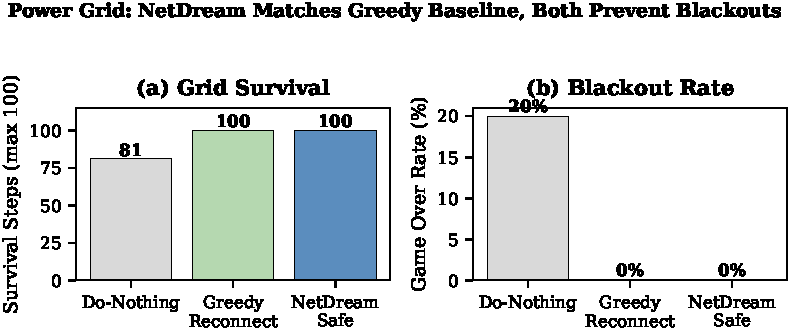
\includegraphics[width=0.55\textwidth]{figures/fig_grid2op_planning.pdf}
\caption{Power grid planning on IEEE 14-bus (Grid2Op). NetDream-Safe
achieves 100\% episode survival and zero overloads, matching the
Greedy-Reconnect heuristic---using the \emph{same} GNN architecture
as K8s with no domain-specific tuning.
Do-Nothing fails in 20\% of episodes due to cascading line trips.}
\label{fig:grid2op}
\end{figure}

\begin{table}[H]
\centering
\small
\caption{Power grid planning results (mean $\pm$ std over 3 seeds).}
\label{tab:full-grid}
\begin{tabular}{@{}lccc@{}}
\toprule
Agent & Survival Steps & Overloads & Game Over (\%) \\
\midrule
Do-Nothing & $81 \pm 39$ & $0.4 \pm 0.8$ & 20\% \\
Greedy-Reconnect & $\mathbf{100 \pm 0}$ & $\mathbf{0.0 \pm 0.0}$ & \textbf{0\%} \\
\textbf{NetDream-Safe} & $\mathbf{100 \pm 0}$ & $\mathbf{0.0 \pm 0.0}$ & \textbf{0\%} \\
\bottomrule
\end{tabular}
\end{table}

On the 14-bus grid, the dominant safe action is reconnection, so
NetDream-Safe and Greedy-Reconnect behave similarly.  The result should
therefore be interpreted as evidence that the architecture learns grid
dynamics, not as a claim of superiority over specialized grid control
heuristics.

Because power grids can be larger than the 14-bus sandbox, we also
test scalability on a 36-bus variant.

\begin{table}[H]
\centering
\small
\caption{Scalability: the same GAT architecture achieves lower prediction MSE
on a larger grid (36 buses, 59 lines) than on the smaller grid (14 buses, 20 lines).}
\label{tab:scalability}
\begin{tabular}{@{}lccc@{}}
\toprule
Grid & 1-step MSE & 5-step MSE & 10-step MSE \\
\midrule
14-bus (14 nodes, 20 lines) & $4.50 \times 10^{-5}$ & $8.65 \times 10^{-4}$ & $5.07 \times 10^{-3}$ \\
36-bus (36 nodes, 59 lines) & $\mathbf{3.30 \times 10^{-5}}$ & $\mathbf{5.94 \times 10^{-4}}$ & $\mathbf{2.30 \times 10^{-3}}$ \\
\bottomrule
\end{tabular}
\end{table}

Having tested an electrical network, we next ask whether the same
planning recipe works in a network governed by pressure dynamics.

\subsection{Water Distribution Control}
\label{app:water}

The second test replaces electrical flow with hydraulic flow.  WaterNet-10
is a pump-controlled water distribution network with one reservoir, two
controllable pump stations, one storage tank, and six demand junctions.
The constraint is minimum service pressure at all demand nodes.  The
analogy to Kubernetes is direct: both are networked systems where local
actions can prevent or trigger future violations.

\begin{table}[H]
\centering
\small
\caption{WaterNet-10 planning results (3 seeds, 96-step episodes, daily demand).
Constraint: pressure $\geq 20\,\text{m}$ at demand nodes.}
\label{tab:water-planning}
\begin{tabular}{@{}lccc@{}}
\toprule
Agent & Avg.\ energy cost & Avg.\ pressure violations & Notes \\
\midrule
Do-Nothing         & $0.0$             & $96.0$             & All steps violate \\
Always-High        & $144.0$           & $19.0$             & Over-provisioned \\
Greedy-Pressure    & $96.0$            & $59.0$             & Reactive heuristic \\
\textbf{NetDream-Safe} & $\mathbf{92.8\pm2.2}$ & $\mathbf{28.7\pm4.5}$ & Same architecture \\
\bottomrule
\end{tabular}
\end{table}

The result again matches the paper's core intuition: a reactive heuristic
can respond only after pressure falls, while the world model can plan
before the violation boundary is crossed.

NetDream-Safe Pareto-dominates Greedy-Pressure: it uses slightly less
energy and cuts pressure violations by more than half.  This mirrors the
Kubernetes result: planning helps when the model can anticipate how local
actions affect future graph-level constraint risk.

\subsection{Epidemic Control on a Mobility Graph}
\label{app:epinet}

The third test moves from engineered infrastructure to a mobility graph.
EpiNet-20 is a 20-node community mobility graph with discrete-time SIR
dynamics.  Nodes are communities, edges encode mobility, and actions are
intervention levels.  The constraint is an outbreak threshold:
$I_i>0.10$ at any node.  The key difficulty is hub propagation: waiting
until a hub crosses a reactive threshold can be too late.

\begin{table}[H]
\centering
\small
\caption{EpiNet-20 planning results (3 seeds, 60-step episodes).
Constraint: $I_i \leq 0.10$ at all nodes.
\emph{Cost efficiency} = (cost increase over No-Intervention) $\div$
(violations reduced); lower is better.}
\label{tab:epinet-planning}
\begin{tabular}{@{}lcccc@{}}
\toprule
Agent & Avg.\ total cost & Avg.\ violations & Cost/viol.\ efficiency & Notes \\
\midrule
No-Intervention    & $197.3\pm0.1$   & $56.7\pm0.5$ & ---  & Epidemic baseline \\
Greedy-Reactive    & $456.9\pm14.1$  & $51.3\pm0.9$ & $48.1$ & Too late at hubs \\
Always-Strong      & $1200.6\pm0.1$  & $\mathbf{0.0}$      & ---  & Over-intervenes \\
\textbf{NetDream-Safe} & $565.9\pm3.2$ & $\mathbf{41.0\pm10.0}$ & $\mathbf{23.5}$ & Same architecture \\
\bottomrule
\end{tabular}
\end{table}

This final domain is especially useful because the failure mechanism is
visibly graph-structured: hub nodes create delayed cascades, just as
bottleneck services can create downstream latency cascades in Kubernetes.

The gain comes from lookahead.  Greedy-Reactive waits for infection to
become high; NetDream can intervene before a hub-driven cascade crosses
the constraint boundary.  Its cost per violation avoided is roughly
2$\times$ better than the reactive policy.

\paragraph{Takeaway.}
The domains differ, but the control pattern is the same.  Across
Kubernetes, power grids, water distribution, and epidemic mobility
graphs, the same idea recurs: learn graph dynamics, imagine short
futures, reject unsafe plans, and act on the best remaining plan.  The
main paper focuses on Kubernetes, but these results suggest that graph
world models are a broader recipe for safe control in networked systems.

\paragraph{Open problems.}
The results also show what NetDream does not yet solve.  Online model
adaptation is needed when workloads drift far from the training
distribution.  Larger service meshes will require sparse or hierarchical
message passing.  Pod-level planning should be coupled with node-level
autoscaling.  Future safety filters should support multiple constraints,
including tail latency, error rate, fairness, and carbon-aware cost.
Finally, robust evaluation will require longer production traces and more
seeds than are feasible in a short EKS experiment window.


\end{document}
